\documentclass[12pt,a4paper,twoside,openright]{scrreprt}
\usepackage[utf8]{inputenc}
\usepackage[british]{babel}
% print
% \usepackage[bottom=20mm, inner=25mm, outer=20mm, headsep=5mm, headheight=5mm, top=20mm, includefoot, heightrounded]{geometry}
% screen
 \usepackage[bottom=20mm, inner=22.5mm, outer=22.5mm, headsep=5mm, headheight=5mm, top=20mm, includefoot, heightrounded]{geometry}
\usepackage[usenames,dvipsnames,svgnames,table]{xcolor}
\usepackage{graphicx}
\usepackage{caption}
\usepackage{setspace}
\usepackage{enumerate}
\usepackage{adjustbox}
\usepackage[newfloat,chapter]{minted}
\usepackage{tabu}
\usepackage[T1]{fontenc}
\usepackage{amsmath}
\usepackage{ amssymb }
\usepackage{cutwin}
%\usepackage{bm}
\usepackage{url}
\usepackage{centernot}
\usepackage{mathtools}
\usepackage{cancel}
\usepackage{turnstile}
\usepackage{pdflscape}
\usepackage{tikz}
\usepackage{siunitx}
\usepackage[full]{textcomp}
\usepackage[osf]{newpxtext} % osf for text, not math
\usepackage{cabin} % sans serif
\usepackage[varqu,varl]{inconsolata} % sans serif typewriter
\usepackage[bigdelims,vvarbb]{newpxmath} % bb from STIX
\usepackage[cal=boondoxo]{mathalfa} % mathcal
\usepackage{hyperref}
\usepackage[style=ieee]{biblatex}
\usepackage[capitalise]{cleveref}
\usepackage[titletoc]{appendix}
\usepackage[margin=2pt]{subfig}

%code highlighting
\usemintedstyle{tango}
%\renewcommand{\theFancyVerbLine}{{\small \newstylenums{\arabic{FancyVerbLine}}}}
\setminted[elixir]{linenos,frame=lines}

\addbibresource{dissertation.bib}

\crefformat{section}{§#2#1#3}
\Crefformat{section}{Section #2#1#3}

\crefrangeformat{section}{§§#3#1#4--#5#2#6}
\Crefrangeformat{section}{Sections #3#1#4--#5#2#6}

\crefname{appch}{Appendix}{Appendices}

\crefmultiformat{section}{§§#2#1#3}{ and~#2#1#3}{, #2#1#3}{ and~#2#1#3}
\Crefmultiformat{section}{Sections #2#1#3}{ and~#2#1#3}{, #2#1#3}{ and~#2#1#3}

\crefrangemultiformat{section}{§§#3#1#4--#5#2#6}{ and~#3#1#4--#5#2#6}{, #3#1#4--#5#2#6}{ and~#3#1#4--#5#2#6}
\Crefrangemultiformat{section}{Sections #3#1#4--#5#2#6}{ and~#3#1#4--#5#2#6}{, #3#1#4--#5#2#6}{ and~#3#1#4--#5#2#6}


% Uncomment below for version suitable for screens
%\setlength{\oddsidemargin}{-0.4mm}    % 25 mm left margin - 1 in
%\setlength{\evensidemargin}{\oddsidemargin}
%\setlength{\topmargin}{-5.4mm}        % 20 mm top margin - 1 in
%\setlength{\textwidth}{160mm}         % 20/25 mm right margin
%\setlength{\textheight}{237mm}        % 20 mm bottom margin
%\setlength{\headheight}{5mm}
%\setlength{\headsep}{5mm}
\setlength{\parindent}{0mm}
\setlength{\parskip}{\medskipamount}
\renewcommand\baselinestretch{1.15} % thesis format (not needed for techreport)
% don't let large figures hijack entire pages
\renewcommand\topfraction{.9}
\renewcommand\textfraction{.1}
\renewcommand\floatpagefraction{.8}

\newcommand{\mlpos}{}

\newcommand{\exs}[1]{\mintinline{elixir}{#1}}

\newcommand{\todo}[1]{\fcolorbox{red}{white}{\parbox{\textwidth}{\textbf{TODO:} {#1}}}}

\AtBeginEnvironment{minted}{%
  \renewcommand{\fcolorbox}[4][]{#4}}
  
\AtBeginEnvironment{mintinline}{%
  \renewcommand{\fcolorbox}[4][]{#4}}

\makeatletter
\DeclareFontFamily{OMX}{MnSymbolE}{}
\DeclareSymbolFont{MnLargeSymbols}{OMX}{MnSymbolE}{m}{n}
\SetSymbolFont{MnLargeSymbols}{bold}{OMX}{MnSymbolE}{b}{n}
\DeclareFontShape{OMX}{MnSymbolE}{m}{n}{
    <-6>  MnSymbolE5
   <6-7>  MnSymbolE6
   <7-8>  MnSymbolE7
   <8-9>  MnSymbolE8
   <9-10> MnSymbolE9
  <10-12> MnSymbolE10
  <12->   MnSymbolE12
}{}
\DeclareFontShape{OMX}{MnSymbolE}{b}{n}{
    <-6>  MnSymbolE-Bold5
   <6-7>  MnSymbolE-Bold6
   <7-8>  MnSymbolE-Bold7
   <8-9>  MnSymbolE-Bold8
   <9-10> MnSymbolE-Bold9
  <10-12> MnSymbolE-Bold10
  <12->   MnSymbolE-Bold12
}{}

\let\llangle\@undefined
\let\rrangle\@undefined
\DeclareMathDelimiter{\llangle}{\mathopen}%
                     {MnLargeSymbols}{'164}{MnLargeSymbols}{'164}
\DeclareMathDelimiter{\rrangle}{\mathclose}%
                     {MnLargeSymbols}{'171}{MnLargeSymbols}{'171}
\makeatother

\setcounter{tocdepth}{2}



%%% BEGIN DOCUMENT
\begin{document}

\renewcommand{\theFancyVerbLine}{{\small \arabic{FancyVerbLine}}}



\begin{titlepage}
\rightline{\LARGE \textbf{Mateusz Jadczak}}

\vspace*{60mm}
\begin{center}
\Huge
\textbf{An implementation of Google Dataflow in the Elixir programming language} \\[5mm]
Computer Science Tripos -- Part II \\[5mm]
Robinson College \\[5mm]
XX May 2017
\end{center}
\end{titlepage}

% Proforma


{\let\cleardoublepage\clearpage \chapter*{Proforma}} % Start on next side

{\large
\begin{tabu}{ll}
Name:               & \textbf {Mateusz Jadczak}                       \\
College:            & \textbf {Robinson}                     \\
Project Title:      & \textbf {TODO MULTILINE} \\
Examination:        & \textbf {Computer Science Tripos -- Part II, June 2017}  \\
Word Count:         & XX\footnotemark[1]  \\
Project Originators: & Dr Alastair Beresford \& Dr Martin Kleppmann     \\
Supervisor:         &   Dr Alastair Beresford           \\ 
\end{tabu}
}
\footnotetext[1]{This word count was computed
using the \texttt{texcount} tool.
}
\stepcounter{footnote}

\bigskip

\section*{Original aims of the project}

TODO


\section*{Work completed}

TODO

\section*{Special difficulties}

TODO
\newpage
\section*{Declaration}

I, Mateusz Jadczak of Robinson College, being a candidate for Part II of the Computer
Science Tripos, hereby declare
that this dissertation and the work described in it are my own work,
unaided except as may be specified below, and that the dissertation
does not contain material that has already been used to any substantial
extent for a comparable purpose.

\bigskip
\leftline{Signed}

\medskip
\leftline{Date}


%\tableofcontents

%\listoffigures

%\newpage


\chapter{Introduction}\label{ch:intro}

\section{Background}\label{sec:intro:background}

In today's fast-moving world of technology, data is king.
The ability to quickly and flexibly process large, heterogeneous and asynchronous streams of data, is core to many businesses, and this need is only increasing \cite{Yin_2015}\cite{mit_bean_variety}.

Of particular interest are datasets which are inherently unordered and unbounded.
For instance, consider the issue of tracking listen counts of songs on a service like Spotify, where some views may occur on cached data stored offline, and may not be sent to the servers until hours later.
Even more trivially, when operating at a global scale, simple issues like clock skew and network latency mean that we cannot expect data to arrive in-order.

Now, suppose we need to aggregate the track listen events into user sessions, defined as listen events occurring sufficiently close to each other.
The amount of complexity and number of special cases even in this reasonable scenario are too large to consider its implementation with dedicated logic.
There is a clear need for an underlying data model and abstraction in order to sanely manage this kind of processing.

Solutions to this problem have been proposed and implemented in open-source systems such as Apache Storm \cite{apache_storm} and Spark Streaming \cite{spark:zaharia2013discretized}, as well as internally in projects like Google's MillWheel \cite{akidau2013millwheel}.
These projects focus on the concept of \emph{stream processing}---the assumption that the inputs are (possibly unbounded, or never-ending) streams of data.
They apply techniques such as windowing, triggering and watermark tracking to make processing this kind of data possible, but in general fall short on sundry features like scalability and fault tolerance, correctness, expressiveness, richness of windowing features, and others.
The key insight is that these solutions are narrowly scoped for particular problem domains, instead of taking a general approach.

\section{Motivation for the Dataflow Model}\label{sec:intro:motivation}

The issues set out in the previous section drove the development of a new, unified model of data processing at Google ~\cite{Akidau:2015}.
This section simply aims to set out the core motivation behind the model, answering the question, ``Why do we need yet another core tool?''

\begin{figure*}[h]
	\centering
	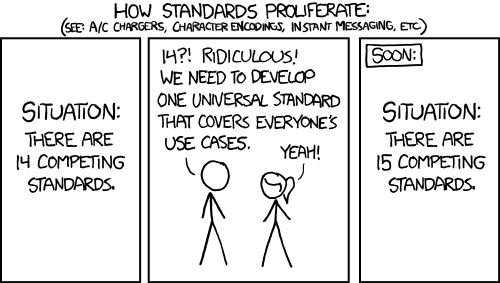
\includegraphics[width=.75\textwidth]{images/xkcd-standards}
	\caption*{\textit{Source: https://xkcd.com/927/\quad(CC BY-NC 2.5)}}
\end{figure*}

Simply put, the Dataflow Model aims to provide a unified way of thinking about data processing, producing a clear, composable abstraction.
It acknowledges the fact that it is impossible to design a perfect (always correct, low-latency and cheap) system, and instead it allows for tunability across these characteristics.

\Cref{sec:prep:dataflow} dives deep into the model itself and explains how these aims are achieved, while \cref{ch:impl} contains a detailed overview of the implementation of the model in practice.

\section{Why Elixir?}\label{sec:intro:elixir}

The Elixir language \cite{Elixir} is relatively young.
It is currently most popular in the web development circles, with many treating it as a Ruby replacement.
How then is this a suitable language in which to implement a robust, complex data processing system?

The answer lies in the underpinnings of the language.
Beneath the shiny, modern exterior lies the battle-hardened BEAM VM and OTP framework, which have been running Erlang-powered systems, mostly in the telecommunications industry, for decades.
We also have at our disposal the entire ecosystem of libraries written for Erlang.

Elixir is a dynamically typed, functional language with no variable mutability and with built-in support for efficiently managing and scheduling hundreds of thousands of \emph{processes} (akin to greenthreads) in a manner which is similar to the Calculus of Sequential Processes.
This invites the use of an actor-based model for applications, and indeed this is the standard approach in the Elixir/BEAM ecosystem.
These built-in primitives allow us to closely implement the desired semantics of the Dataflow Model without the overhead of thousands of lines of scheduling, threading and co\"ordinating\footnotemark[1] code (present in the existing Java implementation).

\footnotetext[1]{
For the typographically observant reader: the \"{} mark in ``co\"ordinating'' is a diaeresis---one of the two diacritical marks which are part of English natively (the other being the grave, as in ``the learn\`ed scholar'').
While its use is uncommon in modern English, some publications (notably The New Yorker) still employ it, and including it is the preferred style of the author.
It is used to indicate that two vowels should be pronounced separately, and not as a diphthong.
}

This project was completed using Elixir v1.4.2, and so all code examples and statements about the language apply to this version, the most current at the time of writing.
\Cref{sec:prep:elixir} gives a brief introduction to the language.



\section{Previous work}\label{sec:intro:previous}
Since the publication of the Dataflow paper \cite{Akidau:2015}, work has been ongoing to implement the Model in practice.
Initially, Google released the Google Cloud Dataflow product \cite{CloudDataflow} along with an SDK to allow users to easily construct data processing pipelines and run them on Google's cloud infrastructure.

In early 2016, Google decided to open-source the project and place it under the care of the Apache Foundation \cite{ApacheDataflowPost}.
This marked the beginning of Apache Beam, a project whose goals were even wider, and include support for cross-platform, cross-language compatibility through separating the creation of the pipelines and their execution on \emph{runners}.

The project has made excellent progress on these fronts, with a fully-featured SDK written in Java as well as a Python SDK.
It is compatible with many data processing systems such as Apache projects Spark, Storm and Flink.
Google Cloud Dataflow remains a paid product capable of running Beam pipelines at scale, but is now only one of many options for doing so.

The implementation also includes an on-machine local runner mainly aimed at testing workflows.
As the simplest yet fully-featured implementation of a Beam runner, it was used as the reference implementation for this project.

Several of the concepts introduced in the Dataflow paper have been used in other projects.
Notably, in the Elixir ecosystem, the Flow project \cite{ElixirFlow} takes some of the concepts---such as the windowing and triggering model---and provides a highly idiomatic way to write and execute multi-threaded computation in Elixir.
Its goals are, however, much narrower than the full Dataflow Model.

Flow has driven the development of GenStage \cite{ElixirGenStage}, a more low-level library implementing demand-driven data flow between actor processes, along with an extensible way to route, partition and dispatch that data.
GenStage forms the backbone of the execution logic in this project, and it is described in more detail in \cref{sec:todo}.

\section{Terminology}\label{sec:intro:terminology}

There are several similar and overloaded terms employed in this dissertation.
This section aims to clarify these and set a convention to be followed.
For a full list of defined terms, the reader should consult the <ref here to Appendix: Glossary>.

Due to the naming change to Apache Beam on open-sourcing the project, the reader will find various references to both the ``Dataflow`` and ``Beam`` on the web with little consistency.

The approach taken in this paper is to refer to the theoretical model described in \cite{Akidau:2015} as the Dataflow Model, and to the current, de facto official, implementation \cite{ApacheBeam} as Beam (generally referred to in full as Apache Beam).
Further, where the ``Beam Model'' is referenced, the author means the Dataflow extended with concepts now found in Apache Beam.
An overview of these is found in \cref{sec:impl:dataflow}.

The virtual machine which powers Erlang and Elixir is called the BEAM.
While efforts are made to refer to the conflicting software in full as the BEAM VM and Apache Beam, the reader should note that wherever the virtual machine is referred to, BEAM appears in all-uppercase form.

\section{Goals and focus}\label{sec:intro:goals}

At the outset, the goal of the project was to write an Elixir-based SDK in order to create Pipelines which could run on the existing Beam software.
Several weeks into the research it emerged concurrently that this approach was impractical to achieve, and that the front-end DSL itself was a relatively small task in itself, not suitable to form the entirety of the project.

The goal then shifted to writing an implementation of a subset of the Beam Model in Elixir.
However, due to the lack of explicit technical documentation of the Model, very quickly it emerged that in order to do this, a very significant amount of work had to be done to reverse-engineer it from an existing open-source codebase and community discussions.
As explained in \cref{sec:impl:dataflow}, many concepts have to be introduced in order to implement the Model, but they are not described directly in any reference material.

Therefore, a second goal of the project emerged, which proved to be a major focus---to extend and clarify the Dataflow Model with the concepts found in Apache Beam, such that a fuller, implementation-ready description is produced.
Once this work was completed, the initial goal of implementing this extended model was achieved with some additional effort.

\section{Results achieved}

Overall, the project was a success, in spite of proving much more challenging than originally imagined.
Due to the highly uncertain nature of the requirements, code had to be continually revisited and improved upon, and evaluation of progress was not straightforward.

Nevertheless, a working implementation of the Model was produced.
The implementation, while forgoing some features, delivered robust performance and a clean programmer interface, meshing well with existing language conventions.

A significant amount of currently non-existent documentation of the theory of the Beam Model was also produced, with some further extensions introduced which solve problems currently being tackled in the Beam Project.



\chapter{Preparation}\label{ch:prep}

\section{The Elixir programming language (a primer)}\label{sec:prep:elixir}

\subsection{Language basics}

\subsection{Concurrency model and the OTP framework}

\section{The Dataflow Model explained}\label{sec:prep:dataflow}

As mentioned in \cref{sec:intro:motivation}, the main feature of the Dataflow model is flexibility.
It aims to create a unified model of data processing which can encompass other processes, placing them in a well-defined structure and allowing the efficient execution of such systems.

It does this by separating the logical notion of data processing from the underlying physical implementation.
An abstract data processing model is defined which covers existing modes of processing by allowing the orthogonal specification of \textbf{what} results are being computed, \textbf{where} in event time they are being computed, \textbf{when} in processing time they are materialised, and \textbf{how} earlier results relate to later refinements \cite[p.~1793]{Akidau:2015}.

This standard model can then be implemented and realised by many different runners, whether natively batch, streaming or hybrid, each with its own set of advantages and disadvantages. 
This flexible approach allows for the tuning of execution technology to business requirements while working with a consistent, expressive theoretical model of the processing itself.

The key takeaway is that this model tries to make as few assumptions as possible on the data inputs, outputs and processes, instead providing simple primitives from which complex system can be constructed.

What follows is a descriptions of the primitive concepts used in the model to more precisely specify all of these properties.

\subsection{``The What'': Transforms and pipelines}\label{sec:prep:dataflow:what}

In the Dataflow model, a \emph{pipeline} is an entire data processing flow.
It may incorporate many different \emph{transforms} which pass data between each other, processing and transforming it as it flows through them.
One can think of pipelines as DAGs\footnote{Directed Acyclic Graphs}, with nodes representing transforms and edges representing the data flowing between them.

\todo{Diagrams of pipelines}

The graph does not have to be connected---it is valid for there to be multiple disjoint data processing paths.
A given transform may produce multiple outputs and it may take in multiple inputs.
It can also produce no outputs, instead causing a side effect such as writing to the network, database or file system.
Transforms can also have no inputs in the graph, instead receiving output from an external source or generating it.
These transforms are called root transforms.

A key advantage of expressing transforms in terms of data flowing is the natural adaptation of the system to unbounded data.
When we say unbounded data, we mean data which may not necessarily have an end.
An example of this may be a stream of events from a website, or the Twitter firehose.
It may help to think of unbounded data as ``streaming'' data, but ``streaming'' and ''batch'' imply execution strategies as opposed to data properties.
Further, in the Dataflow Model it is more convenient to think of all data as being streamed, whether that is a true infinite stream, or merely data being streamed out of a file.

All transforms can be represented fundamentally using only two primitives: \verb|ParDo| and \verb|GroupByKey|\footnotemark[2].

\footnotetext[2]{
Even though these transforms are the only primitives mentioned in the original description of the Model \cite[§2.1]{Akidau:2015}, real implementation will likely special-case several other transforms such as \texttt{AssignTimestamps} or \texttt{Window} and make them primitives for architectural or performance reasons.
}

\todo{diagrams of the transformations performed by these}

\verb|ParDo| represents a flat-map operation---it transforms a data element into zero or more data elements.
The actual computation performed can be arbitrary---the only restriction is that the output depends only on the single element being processed.
This restriction means that the \verb|ParDo| step is ``embarrassingly parallelisable''.
It also translates naturally to operating on unbounded data, as we can emit the output in real-time.

\verb|GroupByKey|, on the other hand, simply groups all key-value pairs into elements with a single key and a collection of elements.
It needs to collect \emph{all} of the data for a particular key before being able to emit its output.
An issue arises when dealing with unbounded data---how do we know when we've received all of the input for a particular key?

To deal with this problem, the Dataflow Model introduces a concept of windowing.

\todo{somewhere we need an explanation of elements' structure as they flow through the pipeline.}

\subsection{``The Where'': Windowing}\label{sec:prep:dataflow:where}

Windowing simply means the additional grouping of elements according to their timestamps in a way which allows us to emit a particular chunk of elements when we know that we have all the data for it.
In the Dataflow Model, we call such a chunk of data belonging to a particular window a \emph{pane}.
Before diving into the details, let us take a brief detour into what ``time'' means in this context.

\subsubsection{Time domains}
We distinguish between two inherent time domains when considering our data as events in time: \emph{event time} and \emph{processing time}.

Event time is the time at which the event actually occurred and is an inherent property of the element itself.
We also refer to this value as the \emph{timestamp} of an element.
Each element in a pipeline must have a timestamp.
We ensure that we have two ``special'' values available, the \emph{minimum} and \emph{maximum timestamps}.
Implementations may make these actual special values, or just use the maximal and minimal values of the underlying representation.

Where there is no inherent time associated with an element (for example it is an un-dated record in a file) or we don't know the timestamp yet (we must process the record before we can extract the timestamp), the element is assigned the minimum timestamp.
The logic of this will become apparent in the following sections.

Processing time is the property of an executing pipeline.
It measures real-world time elapsing as the computation progresses.
The processing time of a particular element at a particular transform is simply the system clock time at which it was seen or processed by that transform.
The Model makes no assumptions about the synchronisation of this time across multiple distributed transforms.

\subsubsection{Types of windows}

\todo{describe global, fixed, sliding and session windowing}

\todo{diagrams showing visually how different windows work}

\subsubsection{Windowing in the Dataflow Model}
The key insight in the Dataflow Model which allows for very flexible windowing is the generalisation of what a window is.

We define the concept of a \emph{windowing function}, which is actually a pair of two functions: \texttt{assign} and \texttt{merge}.

\texttt{assign} takes the timestamp of the element (and optionally the element's data) and outputs a set of windows to which it should be assigned.
This may be a singleton set when windows are non-overlapping, or it could be many windows in the case of e.g.\ sliding windows.
It's important to note that if the element is assigned to multiple windows, we are essentially duplicating that element into each of those windows (since all computation is implicitly grouped by the window).

\texttt{merge} takes a set of windows and optionally merges some or all of them into a new set of windows.
This is used in windowing strategies such as the session windowing mentioned earlier---this function will detect smaller windows near each other and merge them into longer sessions.
Not all windowing functions take advantage of this, and in fact the common strategies apart from session windows are all non-merging.

\todo{diagram / example of how values are transformed with windowing and grouping}

\todo{show an example of the two functions being used to effect session-based windowing}

\subsection{``The When'': Watermarks and triggers}\label{sec:prep:dataflow:when}

In the previous section, we have defined a way to group elements together into windows.
We have also asserted that we can ``emit a particular chunk of elements when we know that we have all the data for it''.
How can we achieve this in light of the fact that data may appear out of order?

The true answer is that we cannot---if we allow the possibility of unpredictably late data in our pipeline, then we cannot ever truly be certain that we can emit a complete pane of data.
What we can do, however, is introduce a model which allows us to specify the desired behaviour in a useful and flexible manner.
Let us first define the concept of \emph{watermarks}.

\subsubsection{Watermarks}

A \emph{watermark} is a lower bound, in event time, on the timestamps of values which have been processed by the pipeline (or a particular transform therein).
For example, if at a particular instant the watermark is time $T$, then we are being promised that all events with timestamps earlier than $T$ have been processed.
A graph of watermark progression against processing time (such as the one in <TODO ref here>) is a useful way to visualise the progress of a pipeline.
Further, this concept allows us to construct a powerful model of lateness in the system.
This is explored further in \cref{sec:prep:dataflow_extra:lateness}.

\todo{diagram of elements being processed in time vs.\ a watermark}

The reader may at this point be asking, ``where does the watermark come from?''
Watermarks in the Dataflow Model are heuristics generated by sources of data, or by user logic in the pipeline.
The exact behaviour is described in \cref{sec:impl:dataflow}.

\subsubsection{Triggering model}

An initial suggestion may be to simply use the watermark as an indication of when a window is finished and is safe to emit; that is, to emit once the watermark has passed the end of the window.
There are two major shortcomings with this strategy:
\begin{itemize}
	\item The watermark may be \textbf{too fast}---we may have decided that all elements for a given window have been seen and emit a pane, only to later on receive a late element which should have been in the window.
	It is unclear what to do with the element in this case.
	
	\item The watermark may be \textbf{too slow}---the heuristic can be too conservative, and even when we have access to the true watermark and not merely a heuristic, a single slow datum can hold up processing for the entire pipeline.
	Therefore using watermarks as the sole signal for emitting data can lead to high latency which may be highly undesirable in some scenarios.
\end{itemize} 

To solve these problems, we define a more complex triggering model.

Firstly, we explicitly allow for data in a particular window to be emitted multiple times.
We call each such emission a pane, and every pane is marked as either early, on time or late.
Secondly, we define a trigger as simply some arbitrary code which has access to time information of elements passing through the transform, as well as watermark and other timing information.
In practice, we define a tree of triggers allowing us to easily achieve desired results (this is explored further in <todo ref>). 

In this manner we can allow for many different behaviours---for example, we may want to receive approximate results (early panes) every ten seconds (in processing time) until the watermark passes the end of the window, at which point an on time pane is emitted.
Any further late data arriving after the watermark can trigger the emission of a late pane.
This, and myriad other combinations, are all possible with this model.
A key strength is that it decouples the marking of data as early/tentative, on time/definitive, or late/corrective, from actually processing the different panes in different ways.

\todo{maybe include a description of a particular use case and which options one would choose for it?}

\todo{one sentence conclusion of triggering / windowing}

\subsection{``The How'': Refinements and retractions}\label{sec:prep:dataflow:how}

While the concepts defined so far allow us to specify when panes should be emitted, we haven't yet settled on what their contents should be, exactly.
We do this by selecting from one of the three refinement modes for a particular \verb|GroupByKey| transform:
\begin{itemize}
	\item The \textbf{discarding} mode simply discards the contents of the window after emitting a pane, such that any new pane emitted will contain only data received since the last emission. There is no relation between the contents of any two panes.
	\item The \textbf{accumulating} mode retains the contents of the window after emitting a pane. A later pane will include all of the data from the initial pane, in addition to any data which has arrived since.
	\item The \textbf{accumulating \& retracting} mode emits retractions to previous panes emitted, as well as following the semantics of the accumulating mode. This means that downstream transforms will first receive notification that the previous pane is now invalid (along with the contents of that pane again, to aid in undoing its results), and after this they will receive the contents of the new pane (which includes the contents of the initial pane, now refined with additional data). 
\end{itemize}

\todo{example of when to use one or the other?}

While the Model broadly defines the concept of retractions and how they may work at a high level, their implementation remains an unsolved problem and is actively being worked on by the Beam project.
The main difficulty lies in the explosion of cached state which seems to be needed in order to allow the undoing of certain operations.
Therefore, the implementation and precise specification of the behaviour of retractions are out of the scope of this paper, and will not be mentioned again.

With the core primitives of the Dataflow Model defined, we will now briefly look at the work done in extending it into a production-ready implementation by the Apache Beam project before considering the additional theory and concepts which must be defined in order to specify the behaviour of such an implementation.

\section{A survey of the Apache Beam project}\label{sec:prep:beam}

The Apache Beam project is a multifaceted undertaking, aiming to build an entire ecosystem around the Model.
The components of the project can be coarsely categorised into SDKs and \emph{runners}.

SDKs provide the user interface to the processing engine.
They are language-specific libraries which allow users to specify the computations to be performed using the tools of their native language, without having to worry about how the computation will be executed.
Currently there is a main, fully-featured Java SDK which serves as the \emph{de~facto} standard implementation.
There is also work being done on a Python version of the SDK.

\todo{``as of the time of writing''?}

SDKs produce descriptions of data processing pipelines in a standard format, which any runner can consume and execute.
This allows the flexibility of being able to select and tune the execution engine orthogonally to the computation itself in accordance with the needs of each user, while keeping a lot of this complexity out of the user-facing data processing model.

As mentioned in \cref{sec:intro:previous}, there is a commercial runner available through Google's Cloud Dataflow product \cite{CloudDataflow} which is a fully-managed, auto-scaling service to execute Beam pipelines.
There are also many runners which utilise other open-source data processing projects, helping to leverage existing resources or run large workloads on-premises rather than in the cloud.

Not all runners support all of the model's features, and the range of support is summarised in \emph{capability matrices}.
A full copy of the official capability matrix can be found in <appendix ref>.

\todo{larger question: is it worth referencing JIRA issues or mailing list discussions? Is it ok to just assert that certain things are the case or are being worked on?}

\todo{include capability matrices? Maybe construct one for this implementation? (https://beam.apache.org/documentation/runners/capability-matrix/)}

A crucial part of the Beam project is the \verb|DirectRunner|---the local on-machine runner provided with the Java SDK.
Its aims are not to necessarily provide a high-performance implementation, but rather to act as the standard implementation of behaviour for other runners to follow.
It is used by users to test out pipelines before sending them to a large-scale runner for production-scale execution.
In fact, much of its functionality is in a separate ``Core'' module, which contains code for other runners to directly use.

This runner is crucial for this project, as it is the result of many man-years of work to come up with a practical implementation of the Dataflow Model while keeping with its definition.
It is the runner whose main focus is model correctness, and as such it is the most appropriate to take as a reference implementation for a project which aims to explore the Dataflow Model, such as this one.


\section{Changing goals}

A side-effect of the way the Dataflow/Beam project has developed is that a large amount of development of the theory of the model has occurred implicitly while the software was worked on.
This happened in place of a formal definition of many concepts, a large amount of which were sketched out in proposals for the project and then iterated upon in code.

Therefore, a huge part of this project was the extraction and reverse-engineering of these concepts from the Java codebase into a more formal specification.
This was further necessitated by the move from an OOP to a functional approach, requiring each concept to be reduced to what it is in the abstract rather than just transferring the class hierarchy to a new language.

The initial project goals did not account for this---it was assumed that a reasonable implementation could be produced from the Dataflow paper \cite{Akidau:2015} using the Beam code simply as reference.


\section{Software Engineering methods}\label{sec:prep:softeng}

\subsection{The spiral model}


This resulted in a need for a highly adaptive and agile development process, since fundamental assumptions made initially changed many times over.

\todo{give actual examples of this happening maybe?}

The Elixir language, with its clear modular structure combined with writing simple, composable functions enabled a flexible model where key logic in the codebase could be refactored with ease when needed.

\todo{summarise spiral model, refer to previous subsection as to why it's good. Include a diagram.}

\subsection{Testing approach}

\todo{mention small, testable modules as well as end-to-end examples}

\section{Starting point}\label{sec:prep:starting}

\todo{Good knowledge of Elixir, and not much more regarding getting to know how Beam ticks inside.}

\section{Summary}\label{sec:prep:summary}

\chapter{Implementation}\label{ch:impl}

\section{The Dataflow Model extended}\label{sec:impl:dataflow}

While the Dataflow paper \cite{Akidau:2015} summarised in \cref{sec:prep:dataflow} gives an overview of the Dataflow Model, it does not provide sufficient detail for its full implementation.
This section draws on many sources, including the Apache Beam codebase, the Apache JIRA issue tracker, and the Apache Beam mailing list in order to compile the extensions to the model necessary for a full, working implementation.

It is important to note that many concepts in the Beam codebase are specific to the Java implementation.
Where the author felt this was the case, a more general concept was defined.
The need to implement these concepts in the highly different Elixir language served as a good benchmark of which concepts were implementation details rather than necessary model changes.
The implementation details of the Elixir implementation are described later in this chapter.

Keeping the previous paragraph in mind, as well as the fact that the Beam project is an active project which is constantly evolving, it is important to note that this chapter does not aim to provide a full description of the Beam Model as it stands today.
Rather, it takes direction and inspiration therefrom to produce a self-consistent extension to the Dataflow Model which enables implementations of it to be built taking a similar approach to Apache Beam.

Finally, the project tackles only the data processing model itself.
Further extensions to the model are necessary, and present in the Beam codebase, in order to enable easy, automated and efficient distribution of execution across a compute cluster.
These include checkpointing, serialisation and partitioning of data, but in themselves form a complex topic worthy of separate discussion.
Nevertheless, these concerns are outside the scope of this project and will only be mentioned tangentially where relevant.

\subsection{Pipelines, Transforms and Collections}

Pipelines are independent ``namespaces'' of computation.
They are essentially DAGs representing the flow of data through the system as it is transformed.

\begin{figure}[t]
	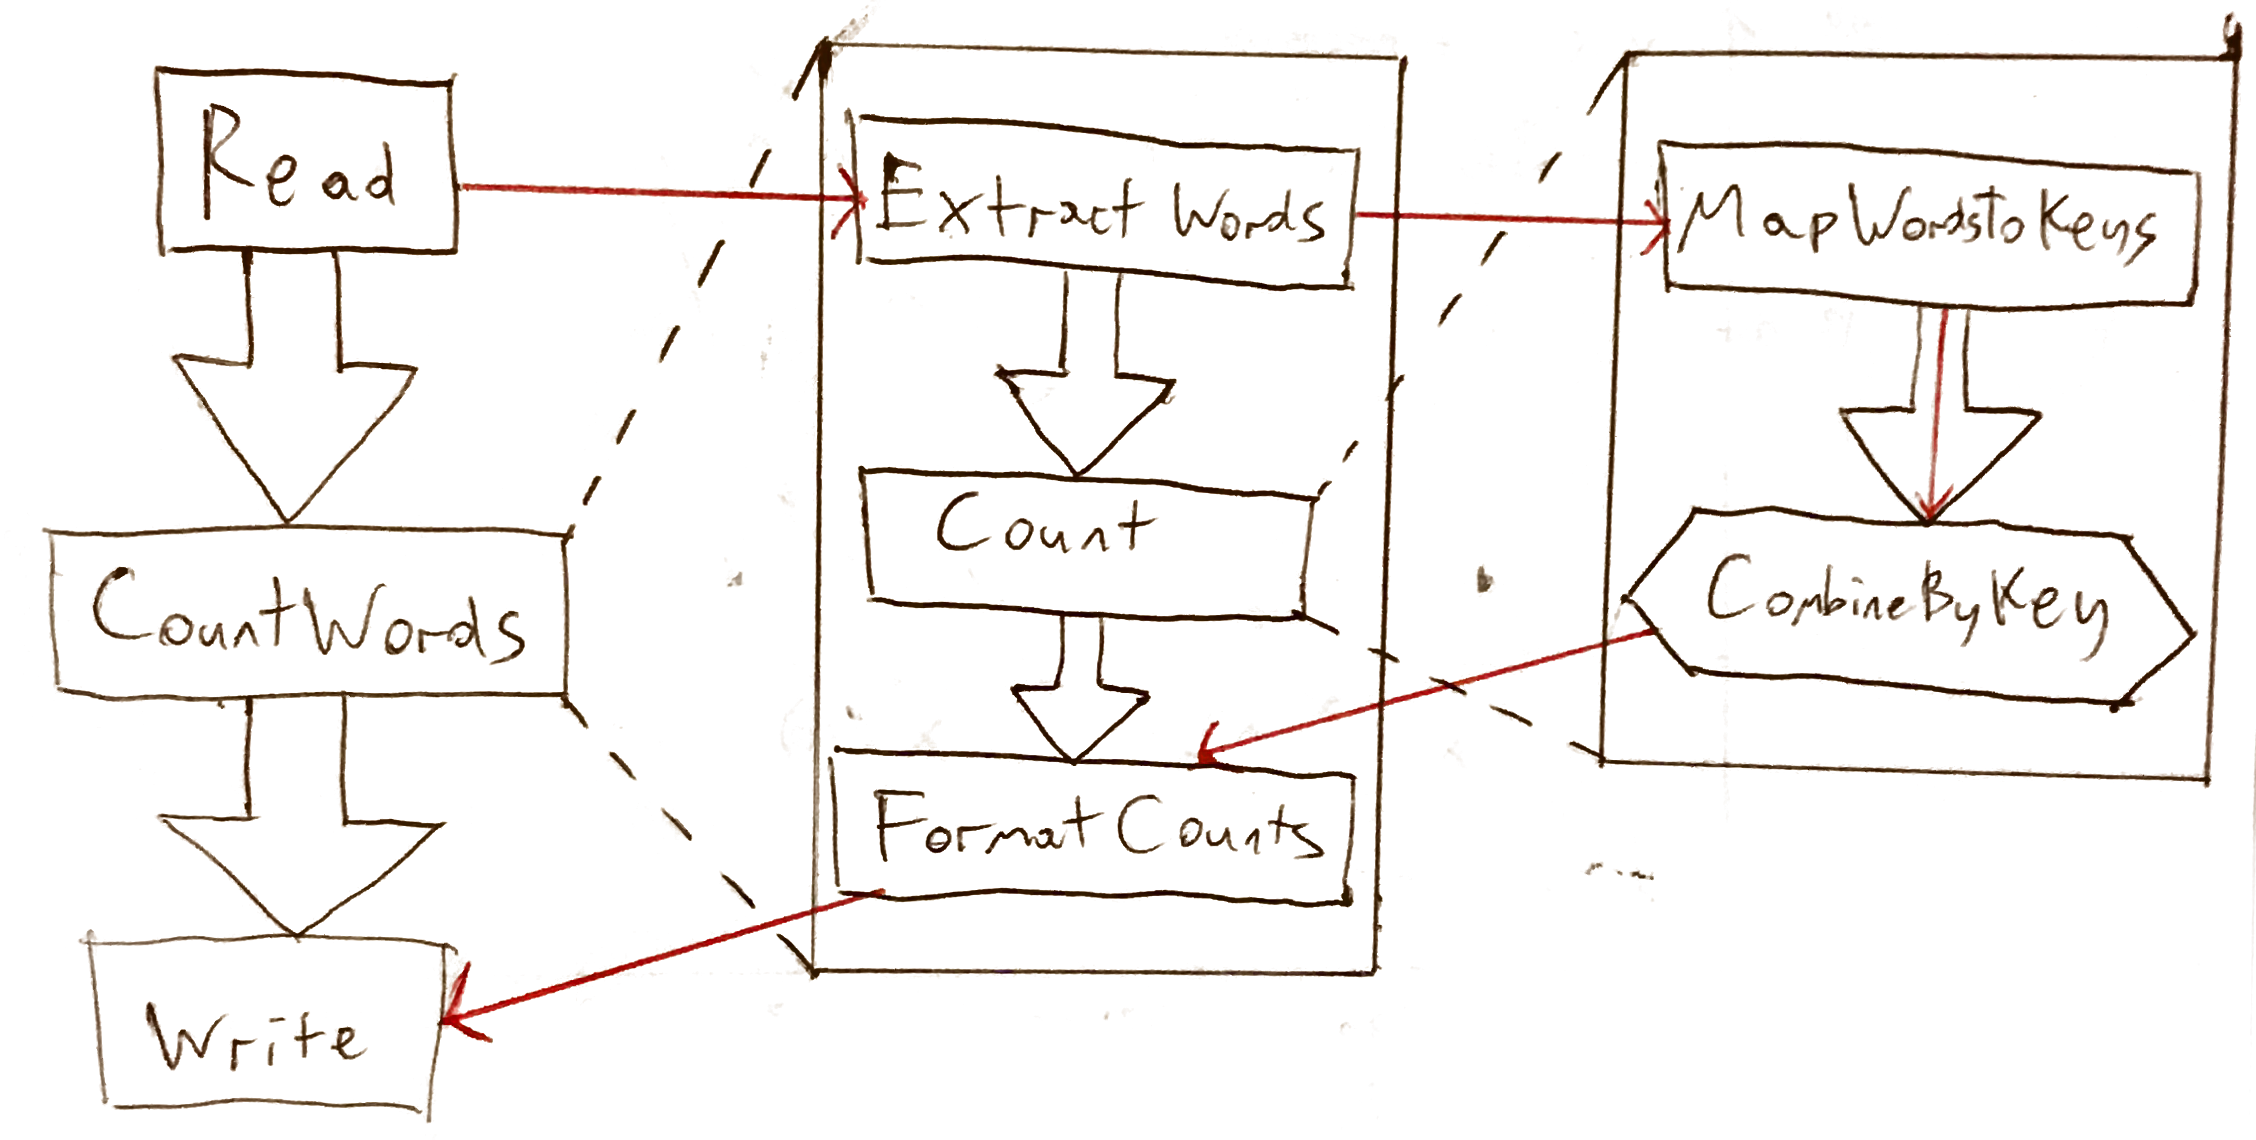
\includegraphics[width=\textwidth]{images/temp/composite-example}
	\caption{An example of a Pipeline utilising composite Transforms. The large arrows indicate the conceptual data flow path. The user expects to see visualisations or statistics using this abstraction. The red edges indicate the actual execution-time data flow---only leaf Transforms are actually instantiated and exchange data.}
	\label{fig:impl:composite-transforms}
\end{figure}

Each node in this graph is a Transform.\footnote
{
In the Beam documentation and various other literature, these objects are called PTransforms and PCollections (with ``P'' standing for ``parallel'').
In this document, they are simply referred to as Transforms and Collections, always capitalised.
}
Transforms can have multiple inputs or outputs.

Each edge in the graph represents a Collection.
This is a notion of the data flowing between Transforms.
Collections can be thought of as the description of all the data that will ever flow out of a particular transform.
The way we construct a Pipeline is by applying Transforms to Collections, the result being another, new Collection (or a structure grouping multiple new Collections).
This Collection encodes various information about the data, depending on the implementation, but among the more important data are the windowing strategy that the collection will follow, used by windowing transforms, which Transform produces the Collection, and the type of the data which will be produced.

Transforms may be primitive or composite---a primitive Transform is directly executed by the pipeline runner, while a composite Transform ``expands'' into multiple sub-Transforms at execution.
This is illustrated in \cref{fig:impl:composite-transforms}.
Different runners may choose to implement different Transforms as primitives and provide composite implementations for the rest.
They do this in a process called \emph{graph surgery}, performed before they start executing the Pipeline.

Composite Transforms are tracked for informational purposes (statistics, logging or visualisation), but don't actually get instantiated at execution time.
The existence of composite Transforms is one of the reasons it is important to track the producer of each Collection---the true producer may be within a nested tree of Transforms rather than being the Transforms we applied directly to the input Collection.


\todo{fix terminology about the below and refactor this section to keep it consistently---easy to get the concepts confused.}

There are three distinct types of entities which could reasonably be called Transforms.
The first is the class instance or structure which holds the parameters for the representation of the Transform and references its code at build-time.
This is what we actually \emph{apply} to a Collection.

The result of such an application is a new Collection.
However, as a side effect, a node representing a particular instance of the Transform in a tree, with particular inputs and outputs, is added to the DAG.
We call such a node an \emph{Applied Transform}.
As well as the parameters of the Transform that was applied, it holds extra information which will be used at execute-time.

Finally, at execute-time, this Applied Transform will be instantiated into some runtime structure which is responsible for actually performing computation.
This may be an object in the case of Java or an actor process in the case of Elixir.
In any case we will call such an instance a \emph{Transform Executor}.

\subsubsection{Collections and streams}

We say that data is \emph{added} to a Collection whenever its producing Transform Executor outputs data.
The Beam implementation explicitly tracks Collections, with Transform Executors really adding data to an in-memory object before it is dispatched as input to other Transform Executors.
The data is groped in \emph{bundles}, which also provide a convenient primitive for serialisation and checkpointing.

The Elixir implementation takes a different approach, with data flowing directly between Transform Executors using message passing.
Collections are used only to set up these links and do not exist at execution time.
The messages sent still contain lists of elements and not individual elements for efficiency.
This is explored further in \cref{todo}.

This illustrates the fact that although we conceptually think of streams of data flowing between Transform Executors, in practice the data is sent and processed in chunks.
The size of these chunks, amongst other factors, can determine where on the spectrum between batch, micro-batch and stream processing a particular runner lies.

\todo{discuss runners somewhere!!}

\subsubsection{Side inputs}

\todo{verify this definition is precise (or don't mention it)}

The Beam implementation has a concept of \emph{side inputs}, which are essentially views of Collections accessible to Transforms to aid in their processing.
For example, a branch of our pipeline processing game messages could identify abusive users and pass the current list as a side input to another Transform which uses this list to remove certain messages from the feed.
This means that the side input is not necessarily a stream of concurrent data as another input would be, but merely a convenient materialisation of data calculated elsewhere.
While being a useful concept, it was not implemented in this project and is not considered further in this document, mostly because of space and time concerns.


\subsection{Windows and panes}

As described in \cref{sec:prep:dataflow:where}, \emph{windows} are a concept used to group elements in event time (i.e.\ with regards to their intrinsic timestamps).
In practice, a window is merely a meta-value acting as a second key by which elements are grouped.
In the Beam and Elixir implementations, only two types of windows are present: the global window, encompassing all time and all elements, and the interval window, encompassing a specific period of time.
The only further requirement we make of a window value is that we be able to obtain the maximal time of an element which is still within that window (the maximal timestamp for the global window, and the inclusive upper bound for an interval window).

\todo{technically it's MAX\_VALUE - 1 in Beam, and special-cased in Elixir. Might not matter.}

What gives the Model its flexibility are \emph{windowing functions}.
A windowing function is simply a collection of two functions which, based optionally on some parameters, are able to \emph{assign} windows to an element based on its timestamp and \emph{merge} multiple windows when needed.
Currently, the only commonly used merging windowing function is the sessions paradigm, described in \cref{sec:prep:dataflow:where}.

\subsubsection{Elementwise and grouping Transforms}

We can draw a distinction between two main types of Transforms---elementwise Transforms and grouping Transforms.
They roughly correspond to the \verb|ParDo| / \verb|GroupByKey| distinction made in \cref{sec:prep:dataflow:what}.

Elementwise Transforms can be thought of as flat-map operations---they take elements and for each one immediately output zero or more other elements.
It is possible for them to keep state, but most model pure functions.
Any state they do keep needs to be appropriately partitioned by key and window, and more complicated Transforms which take advantage of this lay somewhere between the grouping and elementwise paradigms.
Examples of elementwise transforms include \verb|Map|, \verb|FlatMap| and \verb|WindowInto|.

Grouping Transforms perform all operations grouping elements by key and window.
They generally do not output any elements until they are triggered (as described below).
Much of the core complex logic of the Model deals with grouping Transforms and ensuring they produce the correct data at the correct time.
Therefore both of the implementations implement core processing logic for grouping Transforms, only requiring Transform-specific code to be provided, whether as a \verb|ReducingFn| subclass in Java or a \exs{Reducer} module in Elixir, in order to create a new one.
The \exs{ReducingEvaluator} and its associated modules which implement this complex logic in the Elixir implementation are described in \cref{sec:impl:approach}.

\todo{reconsider convention of capitalising Transform. It makes for weird-looking text.}

A \emph{pane} is an element output from a grouping Transform when a trigger fires, representing the output of that Transform for a given key and window.
It generally takes the form of a key-value pair with the value being the output for a particular key.
For example, a simple \verb|GroupByKey| will output panes consisting of a key and a list of values which had that key and were in the given window.
Each pane is marked as early, on-time, or late, and only up to one on-time pane is ever output for each window.

\subsection{Watermarks}

As mentioned in \cref{sec:prep:dataflow:when}, a \emph{watermark} is a promise or heuristic indicating progress in the event stream.
There are several types of watermark used in the Model.

Conceptually, each Collection in the system has a monotonic watermark in event time, called the \emph{global watermark}.
It approximates the point in time up to which the contents of the Collection have been produced.
It is not necessarily actually knowable or able to be computed, either because of the properties of the Collection itself, or because of the distribution of the system amongst remote nodes.

Each Transform may consume (or produce) one or more Collections as inputs (outputs).
The minimum of the global watermarks of its input Collections is the Transform's \emph{global input watermark} ($\mathit{GIWM}$).
Similarly, the minimum of the global watermarks of its output Collections is its \emph{global output watermark} ($\mathit{GOWM}$).
In this way, I/O watermarks extend the notion carried by Collection watermarks to apply to the entire groups of streams Transforms consume and produce.

However, as mentioned above, global watermarks of Collections are not necessarily knowable.
Therefore, we introduce the concept of \emph{local watermarks}, which are scoped to each Transform Executor individually, and which provide us with the proxy through which to observe and control the system.

The \emph{local input watermark} ($\mathit{LIWM}$) of a Transform is a monotonically increasing lower bound on its global input watermark.
Similarly, the \emph{local output watermark} ($\mathit{LOWM}$) of a Transform is a monotonically increasing upper bound on its global output watermark.
This ensures that we always err on the side of treating data as non-late in cases of uncertainty (see \cref{sec:impl:dataflow:lateness}).

It also allows us to simply use the $\mathit{LOWM}$ of one Transform which produces a Collection as one of the components of the $\mathit{LIWM}$ of its consumer.
This means that each Transform receives a $\mathit{LIWM}$ which it cannot control, but can in turn specify its $\mathit{LOWM}$.
It can never (during normal operation\footnotemark) advance its $\mathit{LOWM}$ beyond its $\mathit{LIWM}$ however, because it cannot be sure that it won't receive input data which causes output late with respect to the new $\mathit{LOWM}$.

\footnotetext
{
The exceptions being a Transform at the edge of a watermark domain (\cref{sec:impl:dataflow:wmdomains}) or watermarks being artificially advanced to the maximal timestamp in order to shut down a portion of the Pipeline.
} 

\begin{figure}[t]
	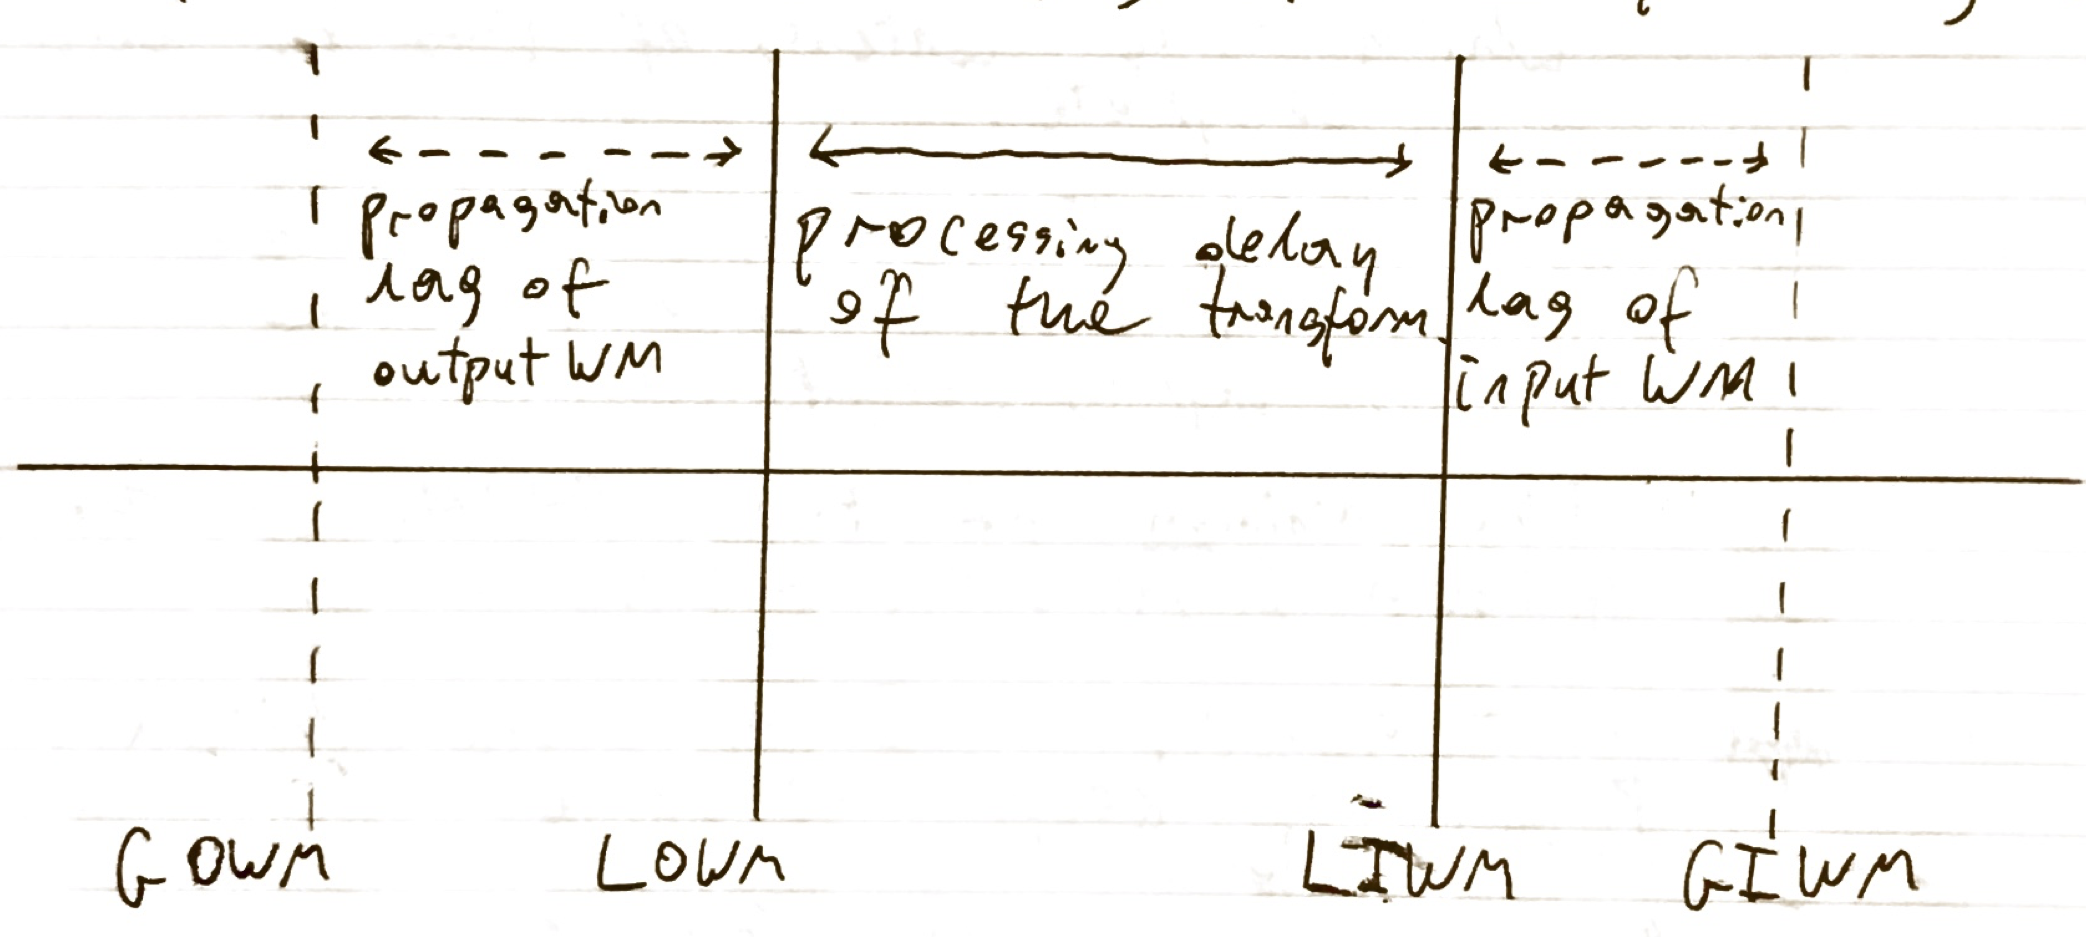
\includegraphics[width=\textwidth]{images/temp/lwm-transform-instantaneous}
	\caption{An instantaneous view of the watermarks of a particular Transform at a single point in processing time.}
	\label{fig:impl:lwm-instantaneous}
\end{figure}

We see that \[ \mathit{GOWM} \leq \mathit{LOWM} \leq \mathit{LIWM} \leq \mathit{GIWM} \] always holds for a particular Transform. \Cref{fig:impl:lwm-instantaneous} illustrates this.

There is also a notion of a \emph{garbage collection watermark}, which is a point in time beyond which it is safe to delete all state we hold about data.
It is usually a constant offset from the local input watermark.
It is not a true component of the Model, but rather an implementation detail necessary to avoid infinitely growing memory consumption.
This concept also limits the amount of lateness we can actually deal with in the system---elements before the GC watermark are silently dropped.
However this is tuneable, so that the user can choose between memory conservation and preservation of late data.

Watermarks provide us with a useful definition of ``doneness''.
In a system where unbounded data may or may not be present, it can be hard to determine when a particular section of the Pipeline is finished and will not receive or output any more data.
We therefore use the watermark to determine this---a watermark of maximal time (infinity) means that we will never receive / output data before that timestamp; since all time is before that timestamp, this implies that we will not receive or output any data at all, and hence we are done.
This is why bounded sources indicate they are done by simply advancing their watermark to the maximal timestamp.

\subsection{``Lateness'' and its semantics}\label{sec:impl:dataflow:lateness}

We have thrown around the term ``lateness'', but so far have failed to define it precisely.
Let us rectify this now.

\todo{evaluate whether using textbf for emphasis is ok or if it's too much}

\textbf{An element added to a Collection is \emph{late} if its timestamp is less than the global watermark of the Collection at the time of the addition, and \emph{non-late}\footnotemark\ otherwise.}

\footnotetext
{
We use \emph{non-late} because such elements could be on-time or early, and we don't care which for the purposes of lateness semantics.
}

We say an element is \emph{droppable} when the the garbage collection watermark is after the end of the window to which it belongs; that is, the data is expired and may be dropped at any further point in the Pipeline.

A key invariant in the Dataflow Model which allows us to easily reason about the behaviour of our system is the following:

\textbf{Only late input can result in lateness anywhere in the system.}

This requirement ensures that we always err on the side of marking data as non-late, and only marking it as late if we are certain that it is.
This is because the goal of the system is to avoid lateness where possible, without holding back the progression of the pipeline.
If we have an opportunity to integrate data which is technically late at one stage of the pipeline into output which is non-late at the next, that is a good thing---it essentially takes advantage of the fact that the later part of a pipeline may be progressing more slowly to allow data to ``catch up'' where possible, while also not holding the progress back to wait for potential late elements.

We can define a set of rules that Transforms in the Model must follow which ensure that the above invariant holds.

A complication arises because we only have access to local watermarks, which are mere approximations of the global watermark, in order to do this.
\Cref{fig:impl:lateness-knowability} illustrates the knowability of whether input or output data is late or not, from the perspective of an individual Transform.

\begin{figure}[t]
	\subfloat[][The knowability of the lateness of $t_{\mathit{in}}$ with respect to the $\mathit{LIWM}$.]{
		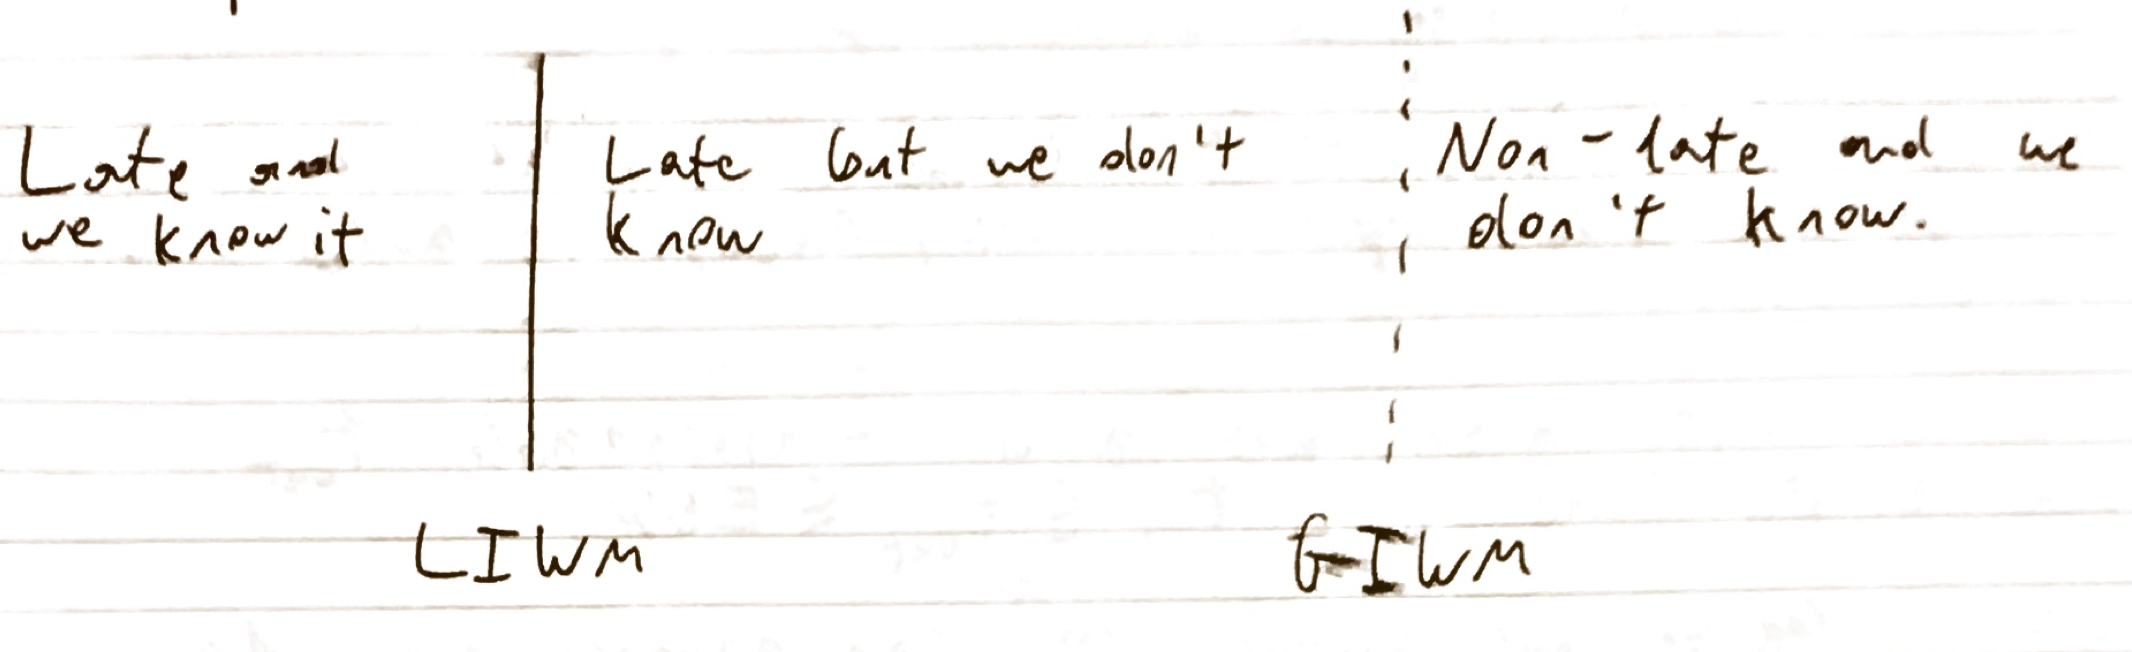
\includegraphics[width=\textwidth]{images/temp/lateness-knowability-input}
	}\\
	\subfloat[][The knowability of the lateness of $t_{\mathit{out}}$ with respect to the $\mathit{LOWM}$.]{
		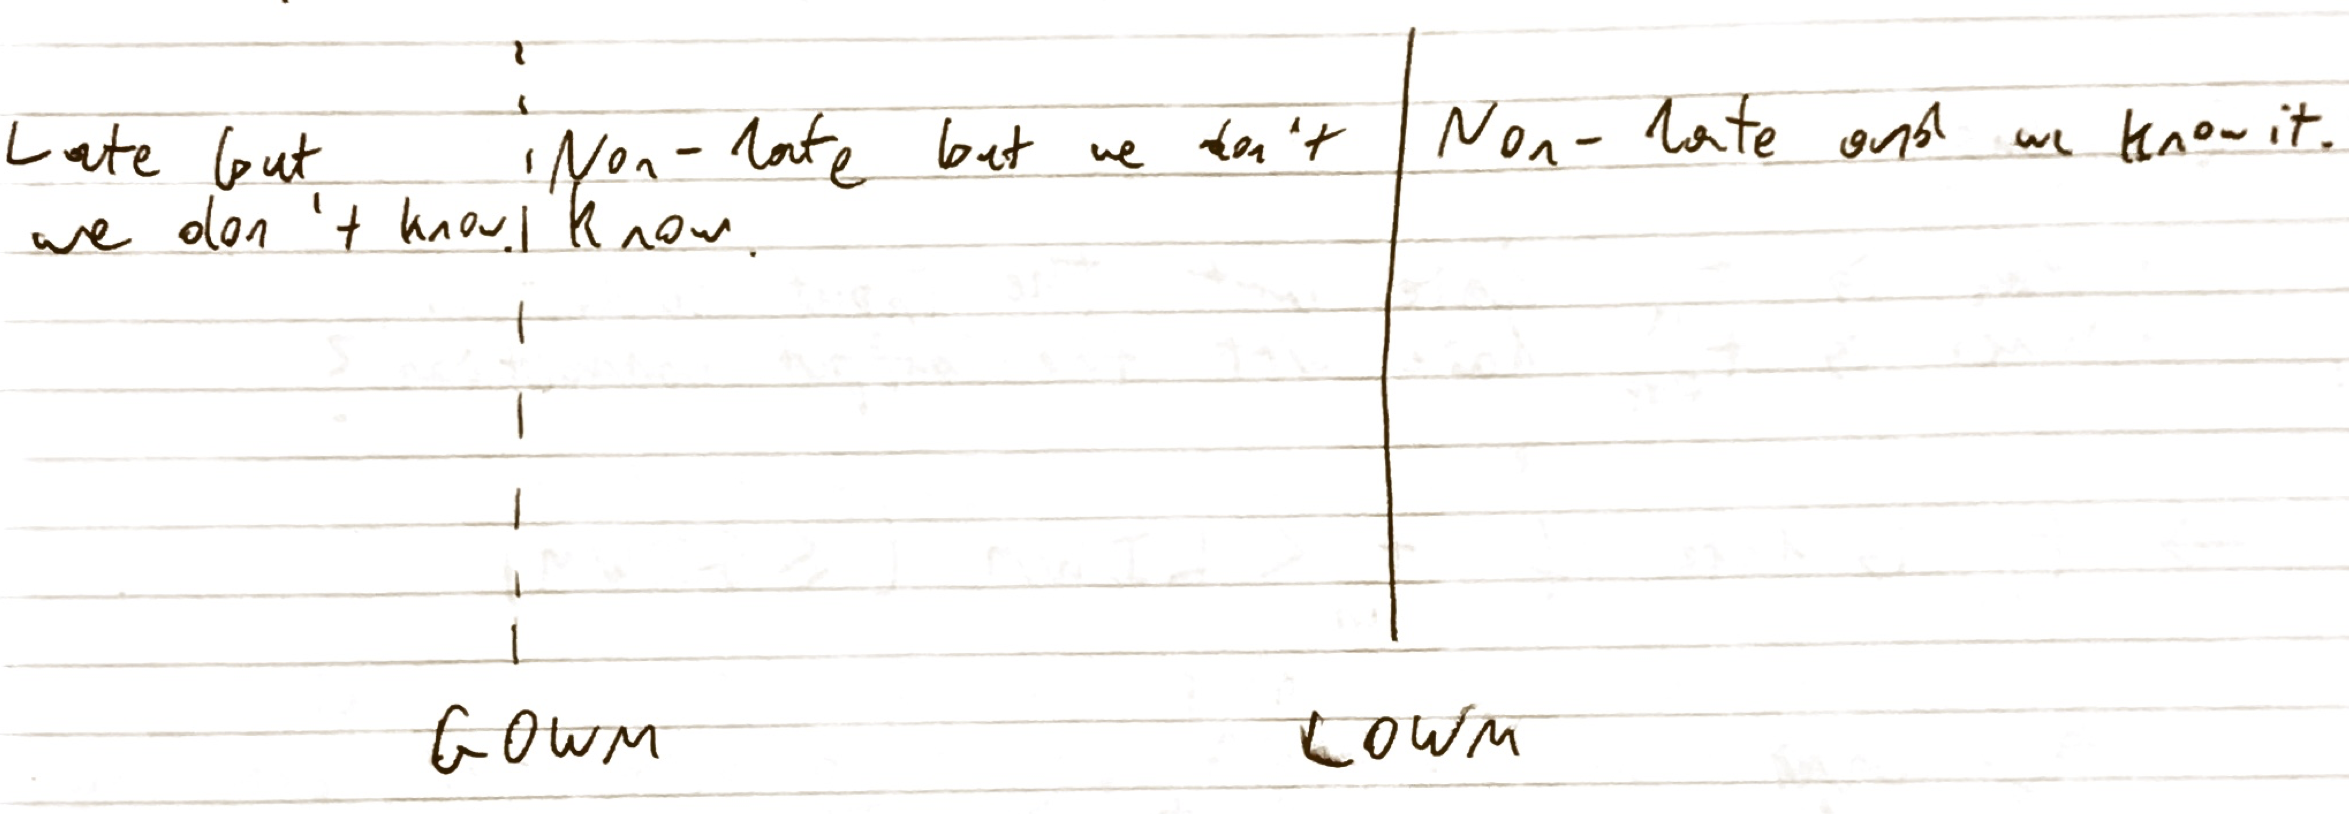
\includegraphics[width=\textwidth]{images/temp/lateness-knowability-output}
	}
	\caption{Diagram illustrating the knowability of the lateness of elements with respect to their position relative to local watermarks.}
	\label{fig:impl:lateness-knowability}
\end{figure}


We therefore expand the original invariants to the following, which ensure the original invariant it is maintained in the situation of imprecise knowledge of the true watermark.

\todo{do we need some sort of informal proof that these actually ensure the original one?}

We then impose the following invariants / requirements on Transforms:
\begin{itemize}
	\item If an element is added to an input Collection non-late, output derived from that element must be added to its respective Collection non-late.
	\item If an element is added to an input Collection non-droppable, then output derived from that element must be added to its Collection non-droppable.
	\item If a pane is emitted, it should not be droppable.
	\item The panes of a window must follow the sequence \verb|EARLY* ON_TIME? LATE*| (zero or more early panes, then zero or one on-time panes, then zero or more late panes).
	\item If a pane is marked early or on-time, it must be non-late in actuality.
	\item If a pane is marked late, it must have been derived \textbf{exclusively} from late input elements.
\end{itemize}

\subsection{Elementwise Transforms}

\todo{describe ParDo and DoFns}

\subsection{Grouping Transform semantics}

\todo{if short on space, move the details of this section to an appendix, but keep only overall decisions/priorities, and the motivations. This is probably a prime candidate for shortening anyway.}

Keeping in mind that the overall goal is to allow the output watermark to progress as fast as possible without introducing any lateness which was not introduced at the source, an overview of the algorithm every grouping Transform must follow can be defined.

Suppose that we have received an element with timestamp $t_{\mathit{in}}$ which belongs to a particular window $w$ with inclusive upper bound $t_{\mathit{EOW}}$, and it is abut to be buffered for output at a later stage.
The element also has a time $t_{\mathit{out}}$, from which the timestamp of the pane this element will be part of is derived.\footnotemark\ 
This time is such that \[t_{\mathit{in}} \leq t_{\mathit{out}} \leq t_{\mathit{EOW}}\] and is included to allow the advancement of the output watermark even if the current window is not yet ready for output.

\footnotetext
{
Both $t_{\mathit{out}}$ and the derived pane timestamp are controlled by a user-specifiable OutputTimeFn, though in most cases the default of ``use the end-of-window time for both'' is used.
}

For example, with sliding windows, once we are in the context of one particular window (elements can have multiple windows) it is safe to treat the timestamp of an element as the end of the window, because all elements in the window are processed the same and the difference is not observable in the output.
Doing this, however, will allow us to advance the watermark to just before the end of the current window (and new elements in this window will not be late, since we perform the lateness checks on $t_{\mathit{out}}$), allowing earlier sliding windows to close and output their panes with less delay.



We don't want elements that will be output late anyway to hold up the output watermark, except to avoid becoming droppable.

\todo{number the invariants and reference throughout?}

\subsubsection{Lateness}

\begin{figure}
	\centering
	\subfloat[][If $t_{\mathit{in}}$ could be non-late, then $t_{\mathit{out}}$ must be non-late. Similarly, if $t_{\mathit{out}}$ could be late, then $t_{\mathit{in}}$ must be late. If $t_{\mathit{out}}$ is non-late and the $\mathit{LIWM}$ has not reached the end-of-window, $t_{\mathit{out}}$ is on-time.]{
		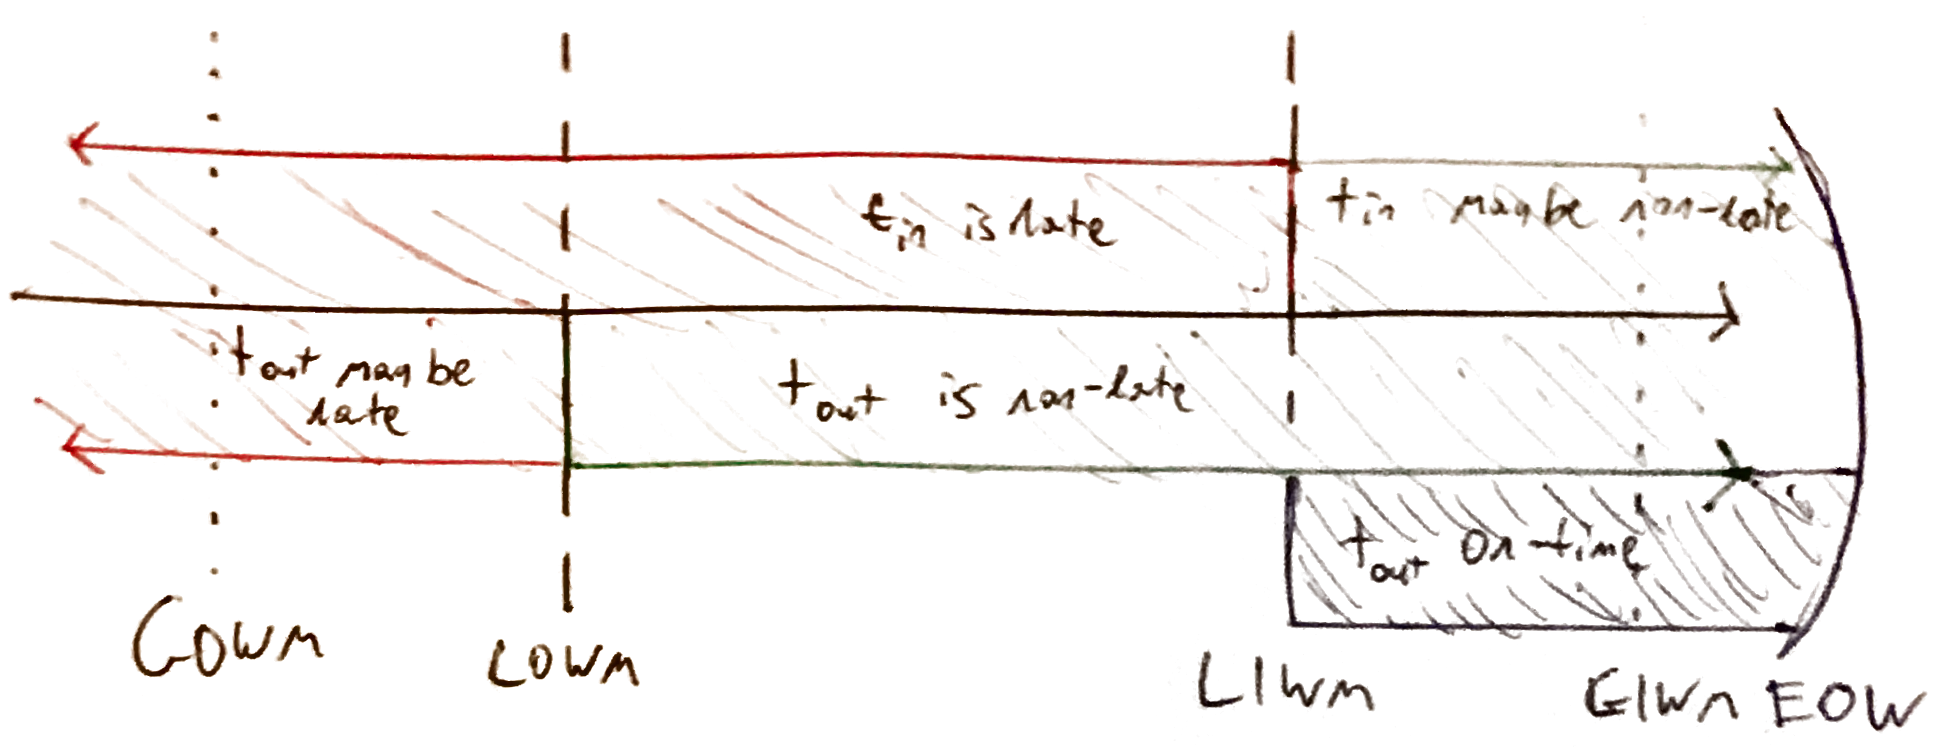
\includegraphics[width=\textwidth]{images/temp/lateness-semantics-1}
		\label{fig:impl:lateness-semantics:a}
	}\\
	\subfloat[][If the $\mathit{LIWM}$ has passed the end-of-window, then $t_{\mathit{in}}$ is definitely late. $t_{\mathit{out}}$ may technically be non-late, but it is not on-time.]{
		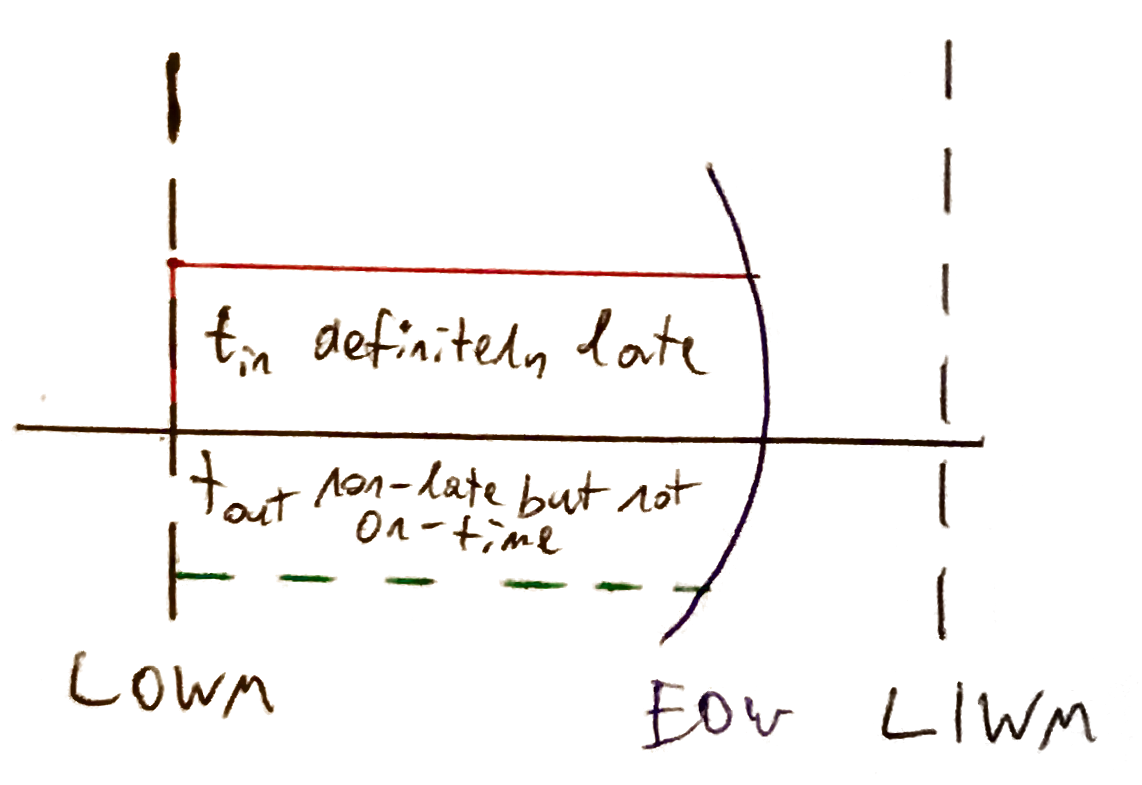
\includegraphics[width=0.5\textwidth]{images/temp/lateness-semantics-2}
	}
	\caption{Diagrams showing regions in event time associated with particular late/non-late or on-time knowledge of $t_{\mathit{in}}$ and $t_{\mathit{out}}$.}
	\label{fig:impl:lateness-semantics}
\end{figure}

There are two questions to answer in order to proceed:
\begin{enumerate}
	\item When is $t_{\mathit{in}}$ late with regards to the input Collection?
	\item When is $t_{\mathit{out}}$ late with regards to the output Collection?
\end{enumerate}

Referring to \cref{fig:impl:lateness-semantics}\subref{fig:impl:lateness-semantics:a} we see that
\begin{enumerate}
	\item \begin{itemize}
	\item $t_{\mathit{in}}$ \textbf{is late} if $t_{\mathit{in}} < \mathit{LIWM}$.
	\item Otherwise, if $t_{\mathit{in}} \geq \mathit{LOWM}$, $t_{\mathit{in}}$ \textbf{could be late} (but we don't know).
	\end{itemize}
	\item \begin{itemize}
	\item $t_{\mathit{out}}$ \textbf{is non-late} if $t_{\mathit{out}} \geq \mathit{LOWM}$.
	\item Otherwise, if $t_{\mathit{out}} < \mathit{LOWM}$, $t_{\mathit{out}}$ \textbf{could be late}. However, in this case, $t_{\mathit{in}}$ \textbf{is definitely late} since $t_{\mathit{in}} \leq t_{\mathit{out}} < \mathit{LOWM} \leq \mathit{LIWM}$.
	\end{itemize}
\end{enumerate}

Note that when $t_{\mathit{in}}$ is late, but $t_{\mathit{out}}$ is non-late, and also $\mathit{LIWM} \leq t_{\mathit{EOW}}$, it is valid with respect to our invariants to treat $t_{\mathit{out}}$ as either late or non-late.
We revisit this choice later.

We have a further requirement for the behaviour of our grouping Transform.
We want to be sure to fire at most one on-time pane.
It \textbf{must} contain all non-late input data up to the end of the window.
It could also contain some late input data which luckily arrived before we emitted the pane (but we do not wait for such data).

To allow us to reason about this, we say that $t_{\mathit{out}}$ is \emph{on-time} if it is non-late, and the input watermark has not yet advanced past its $t_{\mathit{EOW}}$, that is the element arrived early enough to be included in the on-time pane.

\subsubsection{Droppability}

We need to determine two further pieces of information:
\begin{enumerate}
	\item When is the input element droppable?
	\item When is the resulting output going to be droppable?
\end{enumerate}

Denote the allowed lateness used to determine the garbage collection watermark as $\delta$.

$t_{\mathit{in}}$ \textbf{is droppable} if $t_{\mathit{EOW}} < (\mathit{LIWM} - \delta)$.\\
$t_{\mathit{in}}$ \textbf{could be non-droppable} if $t_{\mathit{EOW}} \geq (\mathit{LIWM} - \delta)$.\\
$t_{\mathit{out}}$ \textbf{is non-droppable} if $t_{\mathit{EOW}} \geq (\mathit{LOWM} - \delta)$.\\
$t_{\mathit{out}}$ \textbf{could be droppable} if $t_{\mathit{EOW}} < (\mathit{LOWM} - \delta)$.

Now, if $t_{\mathit{in}}$ \textbf{could be non-droppable} then $t_{\mathit{out}}$ \textbf{is} non-droppable, since \[(\mathit{LOWM} - \delta) \leq (\mathit{LIWM} - \delta) \leq t_{\mathit{in}} \leq t_{\mathit{out}}\;\text{.}\]
Also, if $t_{\mathit{out}}$ \textbf{could be droppable} then $t_{\mathit{in}}$ \textbf{is} droppable, since \[t_{\mathit{in}} \leq t_{\mathit{out}} \leq (\mathit{LOWM} - \delta) \leq (\mathit{LIWM} - \delta)\;\text{.}\]

\subsubsection{Watermark holds}

By default, each Transform Executor outputs a watermark which is equivalent to its input watermark, unless the output watermark is held back by a \emph{watermark hold}.
In that case, the output watermark is the earlier of the two.
Watermark holds provide a mechanism by which the grouping Transform logic can hold back the output watermark until it is sure that it can satisfy the invariants described above.

Each Transform Executor has a watermark manager which maintains a pair of two holds (the data hold and end-of-window/garbage-collection hold) per window\footnotemark.
These are maintained separately so that they can be cleared and manipulated individually, but the overall watermark hold is simply their overall minimum.
Two holds are maintained for each window because some of the logic below requires us to know the data-derived hold even if the hold in effect is derived from the window only.

\footnotetext
{
In the Beam implementation, holds (and other per-window concepts) are per-window-per-key for distribution reasons.
}

The data hold is, in effect, a reduction over all the element timestamps seen so far.
The exact reducing function is determined by the OutputTimeFn in use.
While the default one simply sets all element timestamps to the end of their window---therefore making a reduction redundant as all inputs are always the same---other strategies are available such as ``use the latest timestamp seen so far''.

\todo{diagrams diagrams diagrams}

The EOW/GC hold is a ``fallback'', used when we try to set a hold which cannot be honoured because either the output watermark has already progressed past it, or the input watermark has progressed beyond the EOW and therefore a timer to clear this hold won't be fired.
If we try to set an element hold in either of those situations, we automatically instead try to set the EOW/GC hold instead.

An end-of-window hold is set in two situations:
\begin{itemize}
	\item The element is too late with respect to the output watermark to hold it back, but it may still be possible to include the element in an on-time pane.
	The EOW hold is placed to ensure that pane will not be considered late downstream.
	\item We must ensure that an on-time pane will be emitted for all windows which saw at least one element, even if that on-time pane is empty.
	Therefore, we place the EOW hold to ensure that this (possibly empty) pane will not be considered late downstream.
\end{itemize}

If the input watermark has progressed beyond the end-of-window, we can no longer place the EOW hold since a timer will not fire to clear it.
Instead, if the allowed lateness is non-zero, we try to set an additional garbage collection hold, which is analogous to the end-of-window hold but ensures that the panes we emit are at least non-droppable in the case they must be late.

When the trigger for a window fires, the hold for that window is cleared.
However, a garbage-collection hold may still remain for reasons described above.

It is important to keep in mind that when we talk about ``placing a hold'' below, we actually \emph{attempt} to place an element hold with a particular timestamp, at which point the above checks are performed and the appropriate hold set (or, possibly, no hold is set).
This allows for a decoupling of concerns in the two pieces of logic.

\todo{I do actually think I should reference back to the invariants at each step, saying why it is necessary to maintain them.}

\subsubsection{Transform behaviour}

A grouping Transform does not output panes on receiving input elements, but only when it is triggered.
It can, however, modify its output watermark on receiving elements, and managing this well is crucial to achieve good progress in the Pipeline.

The priorities it adopts, therefore, are:
\begin{itemize}
	\item if it is possible to output data non-late, do that as much as we can;
	\item if process late data and may output late, hold the local output watermark as little as possible (allow it to progress as far as possible);
	\item ensure that the invariants hold and that only a single on-time pane is output.
\end{itemize}

We introduce yet another timestamp for each element, the emission timestamp $t_{\mathit{emit}}$.
It is the timestamp that we actually input into the combination function of the OutputTimeFn to obtain the final timestamp of the resultant pane $T_{\mathit{emit}}$.
This additional transformation affords us the flexibility to combine late data with non-late data to obtain a non-late result.
We require that $t_{\mathit{out}} \leq t_{\mathit{emit}} \leq t_{\mathit{EOW}} + \delta$ where $\delta$ is the allowed lateness.

On receiving each element, then, the Transform Executor must decide:
\begin{itemize}
	\item should the element be dropped?
	\item what hold should be placed on the local output watermark? (see remark above)
	\item what value will be used for $t_{\mathit{emit}}$?
\end{itemize}

\textbf{Case 0: $t_{\mathit{EOW}} < (\mathit{LIWM} - \delta)$}\\
Drop the element.
Since $t_{\mathit{in}}$ and $t_{\mathit{out}}$ are both within the window, they are both certainly droppable and therefore so is the element.

\textbf{Case 1: $t_{\mathit{out}}$ is on-time}\\
We treat the element as non-late.
We set $t_{\mathit{emit}} \coloneq t_{\mathit{out}}$ and place a hold at $t_{\mathit{out}}$.

\textbf{Case 2: $t_{\mathit{out}}$ is not on-time}\\
This is either because $t_{\mathit{out}}$ is possibly late, or because the on-time pane may have already fired.
In either case, $t_{\mathit{in}}$ is definitely late.

We set $t_{\mathit{emit}} \coloneq t_{\mathit{EOW}}$, attempting to shift the element forward in order to possibly include it in an on-time pane.
We could also use the current output watermark for $t_{\mathit{emit}}$, but this would have the effect of significantly holding back watermark progress.
The watermark hold logic described above ensures that the hold is set at $t_{\mathit{EOW}} + \delta$, ensuring we won't produce a droppable pane.

\Cref{fig:todo} illustrates the two situations that are possible in this case. It can be seen that $t_{\mathit{emit}}$ will, in general, be late once emitted, but never be droppable. 
The timestamp used is the latest for the correct window, and the hold used is the latest that prevents dropping.
In this way we allow the watermark to progress in the presence of late data, while ensuring it doesn't become droppable in the process.

\subsubsection{Labelling panes}

\todo{make a typographical distinction between the labels EARLY, ON\_TIME, LATE and the late / non-late state of the elements themselves.}

\todo{explain why the labels are needed and how they're used.}

When a grouping Transform Executor is triggered and outputs a pane (again, simply an element of the output Collection), it must label it as either early, on-time or late.
It does this based on the state of the watermarks and $T_{\mathit{emit}}$, the combined output timestamp determined by the OutputTimeFn from all individual $t_{\mathit{emit}}$ values.
It also determines whether a pane is \emph{final}, which lets the downstream know that no more panes for this window will be emitted (as they would have been emitted droppable).

Since a pane is simply another element, the standard definition of lateness applies.

Therefore if $T_{\mathit{emit}} \geq \mathit{LOWM}$, it is non-late.
By design, every $t_{\mathit{out}}$ that went into the pane was non-late as well.

If $T_{\mathit{emit}} < \mathit{LOWM}$, it is possibly late (it could be on either side of the $\mathit{GOWM}$).
By design, this means that at least some of the $t_{\mathit{out}}$ were treated as late, meaning the corresponding $t_{\mathit{in}}$ were certainly late.
In this case, it is appropriate to output this pane element late and label it late if we need to.

The pane can be marked on-time if $T_{\mathit{emit}}$ is non-late, and if $\mathit{LIWM} > EOW$.
This is because any elements which come in after this condition holds will be treated as late, meaning that they do not need to be included in the on-time pane.
They may still be included in this pane if they arrive before we output it, but we do not have to wait for them, since they were produced late to begin with.

The pane is marked final if $\mathit{LIWM} - \delta > t_{\mathit{EOW}}$, since any incoming elements after this condition starts to hold will just be dropped.

Therefore the pane is labelled as follows:
\begin{itemize}
	\item If $T_{\mathit{emit}}$ is possibly late, label it late.
	\item If $T_{\mathit{emit}}$ is non-late, label it on-time is possible, and early otherwise.\footnotemark
	\item Additionally, label the pane as final if appropriate.
\end{itemize}

\footnotetext
{
Note that in the presence of window merging, two or more on-time panes may end up being emitted for the same data.
The ``one on-time pane'' condition holds only per unique window, and so once the window is merged to become another window, the condition holds separately for this new window.
}

\subsubsection{OutputTimeFn}
Grouping Transforms aggregate element data into an output value.
They must also aggregate the elements' timestamps into a single timestamp used for the output pane.
This concern is often orthogonal to the type of data transformation being performed, and so the Model allows its specification orthogonally, through the use of OutputTimeFns.

An OutputTimeFn specifies three aspects of the aggregation:
\begin{enumerate}
	\item how $t_{\mathit{in}}$ maps to $t_{\mathit{out}}$;
	\item how multiple $t_{\mathit{emit}}$ timestamps combine to give the pane timestamp $T_{\mathit{emit}}$;
	\item how multiple tentative $T_{\mathit{emit}}$ values are combined when two windows merge.
\end{enumerate}

There are two obvious approaches for the first aspect---the identity mapping and simply shifting element timestamps to the end of their window.
Other mappings may also be useful.
For example, when using sliding windows we could shift timestamps just past the end of the previous sliding window, allowing it to close.
The default behaviour in general is to output at the end of the window.

Within a single window, we combine the $t_{\mathit{emit}}$ values generated for each element to obtain the final $T_{\mathit{emit}}$ value for the pane.
An OutputTimeFn specifies an associative, commutative function which can reduce the former to the latter.
It must also ensure that $T_{\mathit{emit}} \geq \max(t_{\mathit{emit}})$ so that non-late inputs are not made late by shifting their timestamps backwards.

The default choice is to, again, use the end-of-window time.
It is simple, efficient and easy to reason about.
However, if the input timestamps are to be stored within the pane and then re-used later by generating new elements with those timestamps, we may use the minimum timestamp of all non-late elements seen so far.
This will hold back the output watermark so that we can once again re-use the input timestamps without them becoming late.

When windows merge, the aggregated pane timestamps must be combined too.
The result of accepting elements into two windows and then merging them should be the same as merging first and then combining new elements into the resultant window.
In general, the merge function either behaves the same as the combination function, or does not use its input at all, again using the end-of-window time (the default).

\subsection{Triggers and timers}

In the previous section, we explored how grouping Transforms accumulate data, ensure that their output watermark is held back until the aggregate is output, and mark their output appropriately to let the downstream know of the type of pane emitted.
However, it is still not clear how exactly they know when they should produce some output at all.

The Model's answer to this is the trigger system.
Triggers were introduced in \cref{sec:prep:dataflow:when}, but this section aims to expand on their semantics and how they function to produce the desired behaviour.

\subsubsection{Triggers as state machines}
Once again, we draw the distinction between triggers at Pipeline-construction time, where they are simply bundles of configuration, and triggers (trigger drivers) at execution-time, where they do real work.
In this second case we can think of triggers as finite state machines; indeed, the Beam implementation places its trigger logic in classes extending \verb|TriggerStateMachine|.

A trigger state machine is instantiated per-window (per-window-per-key in Beam) and is used by the main Transform Executor to make decisions on when to output.
We say that a trigger \emph{fires} when it instructs the Transform Executor to output a pane.
Note that a trigger firing is binary---if it fires, all the currently accumulated data is output into a pane, which is timestamped and marked appropriately as detailed below.

We can easily see the overall behaviour of the FSM by looking at the \exs{TriggerDriver} behaviour from the Elixir implementation in \cref{lst:impl:trigger_driver}.\footnotemark

\footnotetext
{
This listing uses the Elixir behaviour/type syntax. A brief overview is available in \cref{todo}<appendix B>.
}

\begin{listing}[h]
	\begin{minted}{elixir}
defmodule Dataflow.DirectRunner.ReducingEvaluator.TriggerDriver do
  alias Dataflow.Utils.Time
  alias Dataflow.{Trigger, Window}
  
  @opaque state :: any
  @callback init(Trigger.t, Window.t, timing_manager :: pid) :: state
  @callback process_element(state, Time.timestamp) :: state
  @callback merge([state], state) :: state
  @callback should_fire?(state) :: boolean
  @callback fired(state) :: state
  @callback finished?(state) :: boolean
end
	\end{minted}
\caption[The \exs{TriggerDriver} behaviour showing the FSM design of an execution-time trigger.]{The \exs{TriggerDriver} behaviour showing the FSM design of an execution-time trigger. The \exs{timing_manager} passed to the \exs{init} function is the \exs{pid} of the current Transform's timing manager, allowing the trigger driver to set and clear timers and access current watermark state.}
\label{lst:impl:trigger_driver}
\end{listing}

\todo{Consider using the Elixir type syntax everywhere in this chapter to specify the different structures being talked about (instead of prose)}

There we see that the FSM is first initialised (\exs{init/3}) with trigger and window data (along with a handle to a process which allows it to set and clear timers asynchronously, as well as read the watermarks and processing time).
It then receives a series of \exs{process_element/2} calls, receiving the timestamps of elements being processed and being allowed to update its state.
It will optionally be asked to \exs{merge/2} its state with that of other windows---typically we require that the actual trigger being used is the same in all cases.

Note that the trigger driver itself does not asynchronously notify the transform executor of its firing.
Instead, the transform executor will ask the trigger driver if it is ready to fire using \exs{should_fire?/1}.
If so, a pane of output is produced and the trigger driver is notified via the \exs{fired/1} callback.

A trigger is \emph{closed} or \emph{finished} if it will never fire again.
The trigger driver can be asked if it is finished using the \exs{finished?/1} callback.
At that point it is safe to garbage collect the associated window state (including the trigger state itself), leaving only a tombstone indicating that new elements placed in this window should be ignored (since they would never have led to output anyway).

It is clear that this model allows great flexibility in specifying exactly when output should occur.
The FSM can count elements, set timers for particular event or processing times, and flexibly decide if it will fire multiple times.
The model could also quite easily be extended to support punctuations (data-driven triggers) by allowing \exs{process_element/2} to inspect the element value itself.
This is not implemented, but being worked on, in Beam (as certain implementation difficulties arise there) and was considered out-of-scope for the Elixir implementation.

It should be noted that a standard pattern in the Model is to use composite triggers---for example, a trigger which fires when trigger A \emph{or} trigger B fire, or one which takes a one-time firing trigger A (one which becomes finished after firing once) and instead resets it after each firing, making it able to fire indefinitely.
This is enabled by the decouple design of the trigger drivers, allowing them to be queried by a ``parent'' trigger just as easily as they could be queried by the transform executor itself.

\subsubsection{Example: The default trigger}

The \emph{default trigger} used when no other trigger is explicitly specified fires once when the event watermark passes the end-of-window, and fires again every single time a late element is seen (producing a one-element late pane with that element).

\Cref{lst:impl:default_trigger} illustrates the simple logic needed to accomplish this behaviour.

\todo{the listing is about 60 lines of code total including liberal line breaks for readability and comments. possibly skip it here though, maybe just include the pseudocode of the logic?}

\subsubsection{Timers}

Timers are a very simple, but yet flexible way to schedule asynchronous action in the future.
A timer is simply a tuple of \exs{{namespace, time, domain}}\footnotemark, with the \exs{domain} being one of \emph{processing time} or \emph{event time}.
A timing manager is instantiated per transform executor, though it operates asynchronously to the transform executor itself.
It handles watermark management and timers.

\footnotetext
{
In Beam, timers also have a unique ID, in order to identify and compare their identity. This is not needed in Elixir, since they can be directly compared value-wise.
}

Once a timer is set, the timing manager will notify the transform executor once it fires.
This will happen when the input watermark (event time) or clock time (processing time) \textbf{passes} the time of the timer; that is, when the appropriate time measure is strictly greater than the time of the timer.
An exception is a timer for the maximal event time, which fires precisely when that time is reached, since it cannot advance past it.
Multiple timers may fire simultaneously, and the transform executor will be notified of all of them.

The \exs{namespace} of a timer is an arbitrary value, but in practice is used to associate timers to the triggers that set them, or to keep track of different timer purposes in more custom implementations.
Often (e.g.\ in the grouping Transform) the namespace is not even read on a timer firing (all timers are treated the same), but rather only employed to clear specific timers before they fire.

It is important to note that no semantics are implied by the timers themselves---they simply provide a mechanism to receive a notification with a particular identifier at a particular time.
It is up to the transform executor to interpret this and act accordingly.

In the case of a grouping Transform, the executor simply asks the trigger driver whether it should fire already.
The trigger has access to the current watermark state, and so can determine whether it is time to fire.
The flexible implementation means that it could just as well set another timer at this point, enabling strategies such as ``output a pane every five seconds until the end of the window, but only if we've seen 10 elements or more''.

\subsection{Watermark generation and processing}

\todo{diagram}

In \cref{sec:impl:dataflow:lateness} it was asserted that only late input can result in late data anywhere in the system.
Late input was also defined as that whose timestamp falls behind the current input watermark.
The previous sections also detail the exact semantics necessary to preserve watermark correctness along with many useful invariants throughout the whole Pipeline.

However, none of the preceding sections address the question of generating some watermark ``from nothing'' in the first place.
This process is crucial---as mentioned above, it is the only part of the system in which lateness can be introduced.

It also very application-specific.
A watermark is an indication of the progress made so far in the event stream.
For some data sources, we can get a guaranteed-correct position in the stream that we have read up until.
For others, the source provides us with only an approximations.
In yet other cases, we must keep statistics about the source to generate a heuristic ourselves.

Clearly there is no standard solution---there must be a mechanism to allow flexibility in watermark generation.
We introduce the standard concept of a \emph{Source}, which can provide a Collection from some external source when coupled with a \verb|Read| Transform.

At execution, the \verb|Read| Transform Executor will use logic found in the Source it is given in order to assign timestamps to elements being read (usually an intrinsic timestamp in the case of e.g.\ Kafka messages) and to publish a watermark using any logic and state it needs to, with the only restriction being that it must be monotonically increasing.
Bounded sources with no intrinsic timestamps will generally output a minimal watermark (and timestamp all output with the minimal timestamp) until it is finished, advancing the watermark to the maximal timestamp to indicate that.

Sources for popular data sources such as the file system, Apache Kafka, Google BigQuery and others are included in the Beam implementation, and an API is provided to add custom ones with arbitrary watermark logic (in fact, this API is utilised for the example used in \cref{sec:eval:todo}).

\subsubsection{Watermark domains}

Forcing the Source to generate the original input watermark works well from a system perspective, providing a single, easily-managed point where lateness can be introduced.
However, it can cause problems from a user perspective and limit the flexibility of the Model.

Suppose a Pipeline is receiving data containing names of log files being saved off to some cloud storage.
These files contain log entries collected during a particular day, which are then dumped to storage during log rotation every 24 hours.
The timestamp of these elements will be the timestamp of the file, which will be \textbf{after} all of the entries in the file.

This means that if we were to process the file contents in a Transform and output all the log entries within as individual elements, all those elements would have to be output late if they kept their real timestamps.
They could avoid being dropped by selecting an appropriate value for the allowed lateness, but that is a misuse of the Model and semantically incorrect.

In fact, these new elements are not late, because they belong in a different \emph{watermark domain} than the files containing them.
Collections can be thought of as being in the same watermark domain when their elements' timestamps directly relate to one another \textbf{independently of the element data}.
For example, when extracting body text from a social post, it makes sense to assign the same timestamp to the text as was assigned to the post itself.
We don't need to actually look at the post to make that decision.
Similarly, a grouping Transform treats data aggregation and timestamp aggregation orthogonally.

\todo{diagram}

However, in the log-file example given, the timestamp of an individual log entry generated from a file will be dependent on the data of the log entry itself---the recorded time of its generation.
We may be able to provide a guarantee such as ``the timestamp of an entry will never be earlier than 24 hours before the timestamp of a file'', but this again is an application-specific decision, unsuitable for inclusion in a generic Model.
Such a guarantee also constitutes precisely what a watermark is.
Alas, in order to have a predictable lateness model, we have constrained the output watermark of a Transform to always be less than or equal to its input watermark.
Shifting our watermark to 24 hours before the input watermark would violate this invariant.

The solution is to break our Pipeline apart into watermark domains.
The invariants and relationships described in this chapter hold only within one watermark domain---we are essentially treating each one of these as a mini-Pipeline of its own.

Just how event time and processing time are distinguished, we now treat event time as a \emph{class} of domains rather than a single domain of its own.

The lateness semantics only make sense when applied to data which can all be semantically described with one time domain.
Once we switch semantic time domains, there is no general algorithmic solution to obtaining the correct watermark---the problem becomes once-again application-specific.
This is the same problem faced when considering the initial input data into the Pipeline, and so it makes sense that it be solved similarly.

It is to introduce the concept of a Transform which initiates a new watermark domain.
These transforms may directly manage their own input watermark, which does not need to (but can) have a direct relation to their input watermark.

This, of course, introduces a potential source of lateness at every point such a Transform is placed in the Pipeline.
However this also semantically makes sense.
At these points, we are essentially reading a conceptually new, external Collection of elements, with timing information which did not ``exist'' in the Pipeline until this point.
Since this information is unavailable before this point, it is impossible for the previous transformations to have taken account of it in determining whether input to the system was late.

The watermark domain solution is the proposal of the author and is not in place in the Beam Model.
There is no accepted general solution to this problem there.
This solution is implemented in the Elixir implementation of the Model.

The proposed solution also potentially simplifies the original approach to Sources.
Instead of directly coupling watermark management to reading from a Source (which only makes sense for some sources), we can now use general-use Transforms which can provide watermark estimation or transformation algorithms in a standard way in cases where we must generate our own watermarks.

For instance, in the Twitter example in \cref{eval}, the Twitter stream contains no intrinsic watermark information in the metadata---a tweet must be processed to determine its timestamp.
The stream contains no watermark information.

In the Java implementation of the example, a custom Source had to be written which combined responsibility for reading tweets from a network stream, parsing them, extracting a timestamp, and calculating a watermark for the Collection, in one large, tightly coupled class.

In the Elixir version, on the other hand, the root transform only had to worry about reading tweets from the network and parsing their JSON.
It output them with a minimal timestamp and held its own watermark to the minimal timestamp.
A further Transform extracted the timestamp from the data and assigned it to the elements, still in the original domain.
This was valid since timestamps were being shifted forward.
A further yet Transform used the element timestamps to estimate a watermark and output these elements into the new watermark domain.
This Transform was a standard Transform which could be used to estimate the watermark of any stream of timestamped elements.

\todo{consider just moving discussion to the evaluation and reference it here.}


\section{The Dataflow Model implemented}\label{sec:impl:approach}

\subsection{The Dataflow DSL}

An important component of this project, and one of its original goals, was the design of a readable, approachable DSL for constructing pipelines.

As described in \cref{todo}, Elixir has a widely-used pipeline operator \exs{|>}, and programmers are encouraged to express their programs using series of data transformations.
Thus, the Dataflow way of expressing computation translates quite naturally into Elixir, and only a minimal amount of additional syntax is necessary.

\begin{listing}[h]
	\caption{An example of Pipeline construction in Elixir. A Pipeline is created, and to it are applied Transforms which count the words in a file and output these counts to a new file. The Pipeline is then executed.}
	\label{lst:impl:elixir-construct-pipeline}
	\begin{minted}{elixir}
use Dataflow
alias Dataflow.Transforms.{Core, IO, Aggregation}
alias Dataflow.DirectRunner

pipeline = Pipeline.new

pipeline
~> IO.read_file("data/data1.txt")
~> Aggregation.count_elements()
~> "Format Counts" -- Core.map(fn {word, count} -> "#{word}: #{count}" end)
~> IO.write_file("data/output.txt")

DirectRunner.run pipeline, sync: true

	\end{minted}
\end{listing}

\Cref{lst:impl:elixir-construct-pipeline} illustrates the API with a very simple, but working example.
We read a file which contains a single word on each of its lines.
We count the number of occurrences of each word, format this information and output it to another file.

The code is clear and understandable, and maps very well to the Elixir model of data processing.
\Cref{fig:todo} shows this Pipeline as a DAG.

In line 10, we see the \exs{--} operator being used to assign a label to a particular Transform.
Assigning labels to transforms is an important feature, very useful for managing and visualising Pipelines.
This notation evokes the use of \verb|--| to denote a dash in \LaTeX.

\begin{listing}[h]
	\caption{An implementation of the process in \cref{lst:impl:elixir-construct-pipeline} using regular, sequential functions.}
	\label{lst:impl:elixir-normal-comparison}
	\begin{minted}{elixir}
input = File.stream!("data/data1.txt")
output = File.stream!("data/output.txt", [:write])

input
|> count_elements() # helper function
|> Enum.map(fn {word, count} -> "#{word}: #{count}" end)
|> Enum.into(output)
	\end{minted}
\end{listing}

\Cref{lst:impl:elixir-normal-comparison} shows, for comparison, how this process would usually be implemented using normal, sequential processing in Elixir.
The most obvious difference between this listing and \cref{lst:impl:elixir-normal-comparison} is that in the latter, we include an extra \exs{pipeline} identifier which has to explicitly be \exs{run}.
This makes sense, as the Model requires us to separate the description of the computation in the construction phase from its execution in the subsequent phase.

\subsubsection{Using macros}

Those with a passing familiarity with Elixir will recognise that \exs{--} is actually the list difference operator.
While it would be possible to have the \exs{use Dataflow} statement replace the default \exs{--} with a version used for labelling Transforms, it would likely cause confusion.
How then is this entire syntax implemented?

The answer is that \exs{~>} is in fact a macro.
Elixir macros are powerful tools, allowing arbitrary AST transformation at compile time.
They can also cause unexpected behaviour and confusion, and the convention is to keep their use minimal, relying on functions instead.
This is why the definition of \exs{~>} is only a few lines long, shown in \cref{lst:impl:elixir-dpipe-macro-def}.

\begin{listing}[h]
	\caption{The definition of the \exs{~>} macro, showcasing the usefulness and power of Elixir macros.}
	\label{lst:impl:elixir-dpipe-macro-def}
	\begin{minted}[autogobble]{elixir}
 defmacro pvalue ~> transform_with_label do
    case transform_with_label do
      {:--, _, [label, transform]} ->
        quote bind_quoted: [pvalue: pvalue, transform: transform, label: label] do
          Dataflow.__apply_transform__(pvalue, transform, label)
        end
      transform ->
        quote bind_quoted: [pvalue: pvalue, transform: transform] do
          Dataflow.__apply_transform__(pvalue, transform)
        end
    end
  end
	\end{minted}
\end{listing}

Macros are simply functions which, at compile-time, take the Abstract Syntax Trees (ASTs) of their arguments and output an AST with which they are replaced.

The \exs{~>} macro works by pattern-matching on the structure of the second argument, which will either be an AST node of the form \exs{label -- transform} (line 3) or something else (line 7).
The macro outputs a new AST node which simply calls the \exs{Dataflow.__apply_transform__} function which contains the Transform application logic.
This matching at the AST level means that we are free to assign \exs{--} a new meaning only within this expression, without needing to shadow the original meaning for the entire namespace.

Note that we do not have to manually construct this node---the \exs{quote} macro allows us to create one by simply writing syntax and specifying which variables from the macro's environment we want to bind to the environment of the resultant AST node (the \exs{:bind_quoted} option).

The only other piece of ``magic'' present is that the \exs{use Dataflow} line imports the \exs{~>} macro into the top-level namespace so that it can be used straight away.
In fact, that line of code simply calls the \exs{Dataflow.__using__} macro.
In this way, Elixir allows developers to strike a good balance between friendliness and ease-of-use, and the lack of magic and explicitness which is very desirable when things go wrong.

Intuitively, the result of an application of the \exs{~>} operator is a Value, which is either a Collection or some compound (e.g.\ a tuple) containing Collections.
We can hold on to Collections that are returned in this way and apply Transforms to them several times.
This means that we can create branching Pipelines such as the one in \cref{fig:todo} easily, as shown in \cref{lst:impl:diverging-pipelines}.

Note that in order to instantiate a root Transform (one which produces data obtained outside the system somehow), we apply it to the Pipeline itself.

\begin{listing}[h]
	\caption{An example of the creation of a branching Pipeline.}
	\label{lst:impl:diverging-pipelines}
	\begin{minted}[autogobble]{elixir}
pipeline = Pipeline.new

words =
  pipeline
  ~> IO.read_file("data.txt")
  ~> extract_words()
  
# save words to file
words ~> IO.write_file("words.txt")

# also get the top words and write them to another file
words
~> get_top_words()
~> IO.write_file("top_words.txt")
	\end{minted}
\end{listing}

\subsubsection{Structs and protocols}

Since there is a need to separate the construction and execution phases of the Model, the situation cannot be as simple as in \cref{lst:impl:elixir-normal-comparison}, where on passing a value to a ``transformation'', we simply call the function directly.
Instead, we must store the description of the computation in the Pipeline structure.

In order to facilitate this, we make use of Elixir's protocols and structures.
A structure is simply a map with a special \exs{:__struct__} key, which exhibits some special behaviour at compile-time.
A structure is always associated with a particular module.

A protocol is an interface module consisting of a set of functions.
Implementations of a protocol can then be defined on a per-module basis, as long as that module declares a structure.
When the protocol functions are then called with a structure whose module implements that protocol, the actual function called will be dynamically dispatched to that module.

The functions in the example listings, such as \exs{IO.read_file/1}, don't actually perform any computation themselves---instead, they return a structure which stores the arguments passed in and implements the \exs{PTransform.Callable} protocol.
For examples, the result of calling \exs{IO.read_file("data.txt")} is \mintinline{elixir}{%IO.ReadFile{filename: "data.txt"}}.

We then see from the definition of \exs{~>} in \cref{lst:impl:elixir-dpipe-macro-def} that these structures are incorporated into the Pipeline by calling the appropriate function which internally uses the protocol.

The definition of the protocol is presented in \cref{lst:impl:ptransform-callable}.
We see that the only requirement is for the Transform to be able to expand to more Transforms, following the Composite Transforms concept introduced earlier.
Primitive Transforms are not definable by the user and receive special treatment, but the user is free to define their own Composite Transforms by providing an appropriate structure and module, much like one would define small, composable functions.
It is technically possible to simply use a function which composes Transforms internally, but this means that this new Transform is not recognised as a node, leading to a poorer experience once visualisation and/or reporting is introduced.

\subsubsection{Managing DAGs using asynchronous processes}

\todo{ref to a paper on implementing functional dags in Haskell?}

Constructing and working with DAGs in the absence of mutability, especially when advanced functional features such as those found in e.g.\ Haskell are not available, lies somewhere between impossible and infeasible.
Instead of attempting to do this, we leverage the concurrency model of Elixir to simulate a mutable map of Collections and Applied Transforms inside the Pipeline structure.

\todo{mention that Erlang's :digraph library also uses mutable state but is unsuitable for use here?}

The call to \exs{Pipeline.new} actually starts a new process which contains a map of the Collections (edges) and Applied Transforms (nodes) in the Pipeline graph, indexed by a unique integer ID.
This means that it is possible to easily add new structures to the DAG, even in the face of Composite Transforms or branching Pipelines.

It is clear from \cref{lst:impl:diverging-pipelines} that Pipelines behave like mutable objects---merely using the \exs{~>} operator on a Pipeline modifies it.
Therefore Pipelines in this state are better thought of as processes rather than values.
However, once the construction of the Pipeline is finished, it is possible to ``freeze'' it and turn it into a simple data structure which once again behaves in the expected manner.
Indeed, the \exs{DirectRunner.run} function does this internally before taking this data structure and executing it.

\subsection{Making state explicit}

\todo{discuss moving from a stateful approach where things can just grab state out of thin air and mutate it, into an explicit approach of functions taking state and returning a modified version of the state. Also expand on how this forces greater focus on what a particular function actually does as it needs to explicitly receive things it needs, and explicitly return things it touches/modifies.}

\subsection{Managing concurrency with OTP and GenServers}

\todo{Introduce the concept of OTP, GenServers and how they provide robust, serialised concurrency. Make clear how building on top of these core libraries is advantageous and appropriate. Mention how clear semantics enable concurrency design.}

\subsection{The GenStage library}

\todo{Introduce concept of GenStage and how it builds on GenServer. Mention how its operation is a great fit for the type of computation being done in Dataflow.}

\subsection{Extensibility using behaviours and protocols}


\chapter{Evaluation}\label{ch:eval}

Correctness, performance, and ease of use are three important dimensions along which this project was evaluated.

This section outlines the steps taken to test these, and the results obtained.
The data collection and processing methodology is touched upon.
Known limitations in the implementation are also mentioned.


\section{Overall results}\label{sec:eval:overall}

The final project weighed in at approximately 3,200 lines of Elixir code (excluding comments, blank lines and tests).
Approximately 12,000 lines of code were written over the lifetime of the project, illustrating the volatility of the codebase due to evolving requirements.



\section{Correctness testing}\label{sec:eval:correctness}

Unit tests were written for individual modules using the ExUnit library <ref>.

\section{Known limitations}\label{sec:eval:limitations}

This project implements only a core of features from the Beam Model.
There are many known limitations and missing features.
Most of these are due to time constraints in the project, compounded with changing assumptions driving some less-than-optimal decisions earlier in the process.

branching pipelines---need dispatcher\\
side inputs\\
type-checking\\
sessions / unaligned windows in general\\
source/sink API\\


\todo{include capability matrices? Maybe construct one for this implementation? (https://beam.apache.org/documentation/runners/capability-matrix/)}

\section{Approach to empirical evaluation}\label{sec:eval:approach}

\subsection{Test environment}\label{sec:eval:approach:environment}

Efforts were made to collect data in similar environments in order to reduce the potential for uncontrolled variation.

All tests were conducted on a single machine, a MacBook Pro (15-inch, Late 2016) with a 2.9GHz Intel Core i7 CPU and 16GB of 2133 MHz RAM running macOS 10.12.4.
Runtimes used were Elixir 1.4.2 on erts 8.3 and the Oracle JRE v1.8.0\_66-b17.

Prior to conducting the tests, all non-essential background processes and applications were terminated.
Tests were initiated using scripts in order to replicate multiple instances of the tests accurately.

Some of the evaluation (\cref{sec:eval:approach:twitter}) depended on an external stream of data from Twitter.
Due to time constraints and the complexity of the API, it was not feasible to set up a mock server to serve identical data at each execution.
However, informal observation of the data stream show it has a relatively consistent throughput, minimising time-of-execution effects.
Additionally, the tests were executed multiple times throughout the day and the data averaged and aggregated to arrive at the final results, minimising the effects of any variation.

\subsection{Data collection and processing methodologies}\label{sec:eval:approach:collection}


\section{The Twitter example}\label{sec:eval:approach:twitter}

Twitter is a popular social network focused on posting short messages, or \emph{statuses}.
Statuses tend to include \emph{hashtags}, words or short phrases preceded by the \# character.
Hashtags rely on many users using the exact hashtag text in their tweets.
The hashtag can then be used to aggregate and list all of these tweets, perhaps on a particular topic.

It is reasonable, therefore, that an autocomplete functionality may be useful for hashtag entry, to suggest popular hashtags and discourage misspellings.
This real-world scenario formed the basis of this evaluation exercise.

Twitter's free streaming API \cite{TwitterStreamingAPI} was used to receive a stream of English-language tweets on particular topics.
The terms `tracked' to select topics were \texttt{["tech", "technology", "Apple", "Google", "Twitter", "Facebook", "Microsoft", "iPhone", "Mac", "Android", "computers", "CompSci", "science"]}.

The tweets were windowed using sliding windows and then processed further.
Hashtags present were counted per-window.
They were then expanded into all possible prefixes, retaining counts.
Finally, a list of the top three hashtag suggestions for each prefix was produced.
This data could be fed into an autocompletion API, but for the purposes of this exercise was simply printed to console.
\Cref{fig:todo} illustrates the resultant Pipeline.

The scenario provides a good way to test various features of the Model.
Sliding windowing is used, and multiple stages of aggregation per window is employed.
The Pipeline utilises both Elementwise and Grouping Transforms.

The free stream provided by Twitter delivers only around 100 tweets/second.
Therefore, to exercise the systems and compare their performance under load, both Pipelines included a configurable step which duplicated the tweets by a desired factor, simulating a higher-volume stream.

The key success criterion in this example is not necessarily throughput or latency, due to the bounded amount of input and output per window.
Rather, success is defined as being able to deliver results `on time' for each window.

\subsection{Code comparison}\label{sec:eval:code}

The Pipeline was created in both the Java and Elixir implementations of the Model.
The full code is available in \cref{apx:twitter-code}; what follows is a comparison of selected excerpts which illustrate the differences in the two coding styles.

The Java example is noticeably longer, using XX lines of code (excluding blank lines and comments).
In contrast, the Elixir implementation takes only XX lines of code to write.

\subsubsection{Reading tweets}

One of the primary reasons for the length of the Java version is the required method of injecting the stream of tweets into the Pipeline.

\begin{codelisting}
	\caption{Reading a Twitter stream as an unbounded source in Elixir.}
	\label{lst:eval:twitter-readstream-elixir}
	\begin{minted}[breaklines=true]{elixir}
parse_as_timestamp = fn string ->
  string
  |> Timex.parse!("{WDshort} {Mshort} {0D} {h24}:{0m}:{0s} {Z} {YYYY}")
  |> DateTime.to_unix
  |> DTime.timestamp(:seconds)
end
terms = [...]
#...
p
~> "Read Stream" -- IO.read_stream(fn -> ExTwitter.stream_filter(track: terms, language: "en") end)
~> "Extract Timestamps" -- Windowing.with_timestamps(&parse_as_timestamp.(&1.created_at), delay_watermark: {30, :seconds, :event_time})
# `&parse_as_timestamp.(&1.created_at)` is captured lambda syntax for
# fn tweet -> parse_as_timestamp.(tweet.created_at) end
	\end{minted}
\end{codelisting}

\begin{codelisting}
	\caption[Reading a Twitter stream as an unbounded source in Java.]{Reading a Twitter stream as an unbounded source in Java. Code compressed for readability, the full version (\cref{lst:apxb:twitter-java}) is 194 LoC.}
	\label{lst:eval:twitter-readstream-java}
	\begin{minted}[breaklines=true]{java}
static class DummyCheckpoint
    implements UnboundedSource.CheckpointMark, Serializable { /*...*/ }
    
static class TwitterSource
    extends UnboundedSource<Status, DummyCheckpoint> {
    /*...*/
        
    @Override
    public UnboundedReader<Status> createReader(
        PipelineOptions options,
        @Nullable DummyCheckpoint checkpointMark
    ) throws IOException { /*...*/ }

    protected static class Reader
    extends UnboundedSource.UnboundedReader<Status>
    implements StatusListener {
        /*...*/
        private Reader(String[] terms, TwitterSource source) { /*...*/ }
        @Override public boolean start() throws IOException { /*...*/ }
        @Override public boolean advance() throws IOException { /*...*/ }
        @Override public Status getCurrent() throws NoSuchElementException { /*...*/ }
        @Override public Instant getCurrentTimestamp() throws NoSuchElementException { /*...*/ }
        @Override public void close() throws IOException { /*...*/ }
        @Override public Instant getWatermark() { /*...*/ }
        /*...*/
        @Override public void onStatus(Status status) { /*...*/ }
        /*...*/
    }
}
/*...*/
String[] terms = {/*...*/};

p.apply("GetTweets", Read.from(TwitterSource.withTerms(terms)))
	\end{minted}
\end{codelisting}

The Elixir standard library provides a way to deal with potentially unbounded, lazy data---\exs{Stream}s.
As such, it makes sense that one of the Root Transforms provided out of the box in Elixir Dataflow is \exs{IO.read_stream}.
We need only pass a lambda which creates the desired stream on-demand, and its elements will automatically be emitted.

\Cref{lst:eval:twitter-readstream-elixir} illustrates this well.
\exs{ExTwitter} is a Twiter client for Elixir, and indeed it uses the standard \exs{Stream} module to provide its functionality.

Notable is also the ease with which we can timestamp elements based on their data, and assign them a watermark with a simple, standard Transform.
\exs{Windowing.with_timestamps} is a Composite Transform, so it is easy to insert a smarter watermark heuristic if needed; the one used takes the highest timestamp seen so far and outputs a watermark 30 seconds before this---an element can be up to 30 seconds `out of order' before it is considered late.
This showcases the watermark domains feature (\cref{sec:impl:dataflow:watermark-generation}) not present in the Java implementation.
It is possible to decouple the reading of the stream and the timestamp extraction and watermark generation into separate Transforms, resulting in cleaner, more reusable code.

To achieve the same result in Java, we need almost 200 lines of code, as \cref{lst:eval:twitter-readstream-java} summarises.
Firstly, since there is no standard way of representing streaming sequences in Java, custom source of data will need to implement their own asynchronous logic.
\texttt{Twitter4J}, a popular Twitter client library for Java, requires the user to provide a callback object implementing a particular interface to be notified of new tweets.

In order to `connect' the Twitter stream to the Pipeline, an \texttt{UnboundedSource} had to be written.
This is a large interface requiring the implementation of several functions.
Some of these apply to the advanced distributed features offered by Beam such as checkpointing and coding\footnote{
Used to dump data from memory into storage. In Elixir, no extra coding logic is needed since any term can be serialised in a standard way.
} and are omitted.
Others, however, show the incidental complexity present in the Java API.
On top of this, care must be taken to ensure the class is thread-safe.

Since Beam assumes that the entire Pipeline is in the same watermark domain, the Source itself must manage its own timestamping and watermark generation.
In this case, the class must contain logic not only to read, buffer and emit tweets from the network, but also to extract their timestamp and to generate the delayed watermark based on the data.
This results in long, tightly-coupled and complex code.

Clearly, the conventions around \exs{Stream}s in Elixir coupled with the decoupling of reading and processing logic due to the inclusion of watermark domains are a double-whammy which cause Elixir to come out on top in this comparison.

\subsubsection{Lambdas vs.\ classes}

The Dataflow Model adopts an inherently functional model of computation based on functions transforming data, often using standard patterns of mapping and filtering.
Java's support of this model is poor.
This is exemplified best by the common need to specify logic in small internal classes as in \cref{lst:eval:twitter-lambdas-java}.

\begin{codelisting}
	\caption[Using internal classes to specify transformation logic in Java.]{In Java, there is often a need to use internal classes to specify logic. While Java~8 lambdas can be used, the lack of  type inference means that internal classes are often the cleaner solution.}
	\label{lst:eval:twitter-lambdas-java}
	\begin{minted}[breaklines=true]{java}
 public static class GeneratePrefixesFn
 extends SimpleFunction<KV<String, Long>, List<KV<String, KV<String, Long>>>> {
    @Override
    public List<KV<String, KV<String, Long>>> apply(KV<String, Long> tagWithCount) {
        List<KV<String, KV<String, Long>>> result = new ArrayList<>();
        String downcased = tagWithCount.getKey().toLowerCase();
        for (int i = 1; i <= downcased.length(); i++) {
            String prefix = downcased.substring(0, i);
            result.add(KV.of(prefix, tagWithCount));
        }
     return result;
    }
}
public static class DiscardCountsFn
extends SimpleFunction<KV<String, List<KV<String, Long>>>, KV<String, List<String>>> {
    @Override
    public KV<String, List<String>> apply(KV<String, List<KV<String, Long>>> el) {
        List<String> prefixes = l.getValue().stream().map((KV::getKey)).collect(Collectors.toList());
        return KV.of(el.getKey(), prefixes);
    }
}
/*...*/
.apply("GeneratePrefixes", FlatMapElements.via(new GeneratePrefixesFn()))
/*...*/
.apply("DiscardCounts", MapElements.via(new DiscardCountsFn()))
	\end{minted}
\end{codelisting}

\begin{codelisting}
	\caption[Using lambdas to specify transformation logic in Elixir.]{In Elixir, we take advantage of the inherent functional paradigm of the language to specify transformation logic in a familiar way.}
	\label{lst:eval:twitter-lambdas-elixir}
	\begin{minted}[breaklines=true]{elixir}
~> "Generate Prefixes" -- Core.flat_map(fn {tag, count} ->
  len = String.length tag
  for i <- 0..(len-1), downcased = String.downcase(tag),
    prefix = String.slice(downcased, 0..i),
    do: {prefix, {tag, count}}
 end)
# ...
~> "Discard Exact Counts" -- Core.map(fn {prefix, tcs} ->
  {prefix, Enum.map(tcs, fn {tag, _count} -> tag end)}
 end)
	\end{minted}
\end{codelisting}

\Cref{lst:eval:twitter-lambdas-elixir} shows that Elixir, as a functional language, excels at expressing these kinds of computation natively.

\subsubsection{Summary}

Though formal user studies were not performed to assess the `friendliness' or ease of use of the two SDKs empirically, the preceding examples should show at least that Elixir as a language is much better suited to express the concepts of the Dataflow Model in code.
Java's paradigm is orthogonal to the way computation is reasoned about in the Model, and even though a `fluent API' can be used to make things as friendly as possible, the static typing coupled with no type inference fundamentally limits the expressivity of the language in uses like this one.


\subsection{Performance evaluation}\label{sec:eval:performance}

\subsection{Resource consumption}\label{sec:eval:resource}

\section{Latency evaluation}\label{sec:eval:latency}

A key performance indicator of stream-processing systems is their latency when processing streams of data element-wise.
While much of the power of the Model comes from its grouping and windowing facilities, its goal is to subsume many other models of computation, pure stream processing being one of those.

\subsection{Methodology}

In this experiment, a Pipeline was created in which integer elements were generated in a rate-limited fashion and passed through a series of identity Transforms.
The latency of each element from the moment of its generation to its output at the last identity Transform was measured.
The rate of generation of elements and the length of the Pipeline were then varied and the effects of each on the measured latency analysed.


\chapter{Conclusions}\label{ch:concl}

The project achieved its stated goals and is a success.
Success criteria were defined as the `successful execution of test cases specified during the preparation phase' (\cref{sec:eval:latency,sec:eval:twitter:throughput}) and the `provision of a well-reasoned argument backed with code examples of code which is easier to write, understand, and better captures the essence of the Model when written using the Elixir DSL compared to the Java API' (\cref{sec:impl:approach:dsl,sec:eval:twitter:code}).

The project inferred the semantics of the Beam Model using source code, the Apache issue tracker and the project mailing list.
These were described to a level of detail necessary for a working implementation in \cref{sec:impl:dataflow}.

A working implementation of the Model was produced in the Elixir programming language, showing its suitability for developing systems such as this one.
GenStage~\cite{ElixirGenStage}, a low-level library providing a demand-driven data pipelining actor system with backpressure was used as the backbone of the system.

The implementation was evaluated, and though it was built with the aim of functionality, not performance, it displayed excellent performance characteristics when pitted against both the local Beam runner and the optimised Apache Beam runner.
It was able to sustain a sub-\SI{10}{\milli\second} median latency when passing a busy (\SI{100}{\per\second}) stream of elements through a \num{2000}-Transform Pipeline (\cref{sec:eval:latency}).

Its suitability for real-world scenarios was shown by its performance while processing a large stream of tweets to produce hashtag autocomplete suggestions.
Replication techniques were employed to show that Elixir Dataflow can compute hashtag autocomplete suggestions on streams of up to \num{25000} tweets per second---a throughput which would allow it to process all tweets on Twitter ($\sim$\num{7000} tweets per second) three times over~(\cref{sec:eval:twitter:throughput}).

The developer-friendliness of the resultant system was also demonstrated, with a real-world example requiring over \num6$\times$ less code to implement than Java~(\cref{sec:eval:twitter:code}).
The paradigms and conventions of the Elixir ecosystem are a great match for the concepts of the Model (\cref{sec:impl:approach:dsl}).

All Beam implementations lack full support for all of the features (\cref{sec:eval:limitations}) and Elixir Dataflow is no different.
Some of these features---such as branching Pipeline support---would be relatively simple to add but have been omitted due to time constraints.
Further, the implementation forgoes several possible optimisations.
Other implementations have introduced Transform coalescing, where several Elementwise Transforms in sequence can be merged into one which applies the compound operation.
There is also no automatic Transform-level parallelisation, where a Collection is automatically partitioned and processed concurrently.
The lack of this optimisation proved to be the limiting factor when evaluating the Twitter Pipeline throughput.

The seamless distribution of the system across a cluster of nodes would be an important step towards handling production loads.
OTP and the BEAM VM provide fantastic tools and primitives which make the ecosystem an excellent fit for this kind of work, but distributed computation remains intrinsically difficult to control.

Finally, work is ongoing in the Beam community \cite{JIRA-retractions} to develop the semantics needed to support refinements and retractions as described in the original paper.
This is a fundamentally difficult problem to solve without an explosion in the size of cached state.
A general solution to this problem is likely to be an interesting area of research in the future.

\begin{appendices}
	\crefalias{chapter}{appch}
	\chapter{Glossary}
\end{appendices}

\printbibliography[title=References]

% Main document




\end{document}